%%%%%%%%%%%%%%%%%%%%%%%%%%%%%%%%%%%%%%%%
% datoteka diploma-vzorec.tex
%
% vzorčna datoteka za pisanje diplomskega dela v formatu LaTeX
% na UL Fakulteti za računalništvo in informatiko
%
% vkup spravil Gašper Fijavž, december 2010
% 
%
%
% verzija 12. februar 2014 (besedilo teme, seznam kratic, popravki Gašper Fijavž)
% verzija 10. marec 2014 (redakcijski popravki Zoran Bosnić)
% verzija 11. marec 2014 (redakcijski popravki Gašper Fijavž)
% verzija 15. april 2014 (pdf/a 1b compliance, not really - just claiming, Damjan Cvetan, Gašper Fijavž)
% verzija 23. april 2014 (privzeto cc licenca)
% verzija 16. september 2014 (odmiki strain od roba)
% verzija 28. oktober 2014 (odstranil vpisno številko)
% verija 5. februar 2015 (Literatura v kazalu, online literatura)

\documentclass[a4paper, 12pt]{book}

\usepackage[utf8x]{inputenc}   % omogoča uporabo slovenskih črk kodiranih v formatu UTF-8
\usepackage[slovene,english]{babel}    % naloži, med drugim, slovenske delilne vzorce
\usepackage[pdftex]{graphicx}  % omogoča vlaganje slik različnih formatov
\usepackage{fancyhdr}          % poskrbi, na primer, za glave strani
\usepackage{amssymb}           % dodatni simboli
\usepackage{amsmath}           % eqref, npr.
%\usepackage{hyperxmp}
\usepackage[pdftex, colorlinks=true,
						citecolor=black, filecolor=black, 
						linkcolor=black, urlcolor=black,
						pagebackref=false, 
						pdfproducer={LaTeX}, pdfcreator={LaTeX}, hidelinks]{hyperref}
\usepackage{url}
\usepackage{cite}
\usepackage{float}
\usepackage{listings}
\raggedbottom
\graphicspath{ {slike/} }
%%%%%%%%%%%%%%%%%%%%%%%%%%%%%%%%%%%%%%%%
%	DIPLOMA INFO
%%%%%%%%%%%%%%%%%%%%%%%%%%%%%%%%%%%%%%%%
\newcommand{\ttitle}{Večkamerni sistem za lokalizacijo objekta v prostoru}
\newcommand{\ttitleEn}{Multicamera system for object localization in space}
\newcommand{\tsubject}{\ttitle}
\newcommand{\tsubjectEn}{\ttitleEn}
\newcommand{\tauthor}{Ernest Beličič}
\newcommand{\tkeywords}{lokalizacija, triangulacija, računalniški vid, kalibracija kamer}
\newcommand{\tkeywordsEn}{localization, triangulation, computer vision, camera calibration}



\usepackage{hyperref}
%%%%%%%%%%%%%%%%%%%%%%%%%%%%%%%%%%%%%%%%
%	HYPERREF SETUP
%%%%%%%%%%%%%%%%%%%%%%%%%%%%%%%%%%%%%%%%
\hypersetup{pdftitle={\ttitle}}
\hypersetup{pdfsubject=\ttitleEn}
\hypersetup{pdfauthor={\tauthor, ernest.belicic@gmail.com}}
\hypersetup{pdfkeywords=\tkeywordsEn}


 


%%%%%%%%%%%%%%%%%%%%%%%%%%%%%%%%%%%%%%%%
% postavitev strani
%%%%%%%%%%%%%%%%%%%%%%%%%%%%%%%%%%%%%%%%  

\addtolength{\marginparwidth}{-20pt} % robovi za tisk
\addtolength{\oddsidemargin}{40pt}
\addtolength{\evensidemargin}{-40pt}

\renewcommand{\baselinestretch}{1.3} % ustrezen razmik med vrsticami
\setlength{\headheight}{15pt}        % potreben prostor na vrhu
\renewcommand{\chaptermark}[1]%
{\markboth{\MakeUppercase{\thechapter.\ #1}}{}} \renewcommand{\sectionmark}[1]%
{\markright{\MakeUppercase{\thesection.\ #1}}} \renewcommand{\headrulewidth}{0.5pt} \renewcommand{\footrulewidth}{0pt}
\fancyhf{}
\fancyhead[LE,RO]{\sl \thepage} \fancyhead[LO]{\sl \rightmark} \fancyhead[RE]{\sl \leftmark}



\newcommand{\BibTeX}{{\sc Bib}\TeX}

%%%%%%%%%%%%%%%%%%%%%%%%%%%%%%%%%%%%%%%%
% naslovi
%%%%%%%%%%%%%%%%%%%%%%%%%%%%%%%%%%%%%%%%  


\newcommand{\autfont}{\Large}
\newcommand{\titfont}{\LARGE\bf}
\newcommand{\clearemptydoublepage}{\newpage{\pagestyle{empty}\cleardoublepage}}
\setcounter{tocdepth}{1}	      % globina kazala

%%%%%%%%%%%%%%%%%%%%%%%%%%%%%%%%%%%%%%%%
% konstrukti
%%%%%%%%%%%%%%%%%%%%%%%%%%%%%%%%%%%%%%%%  
\newtheorem{izrek}{Izrek}[chapter]
\newtheorem{trditev}{Trditev}[izrek]
\newenvironment{dokaz}{\emph{Dokaz.}\ }{\hspace{\fill}{$\Box$}}

%%%%%%%%%%%%%%%%%%%%%%%%%%%%%%%%%%%%%%%%%%%%%%%%%%%%%%%%%%%%%%%%%%%%%%%%%%%%%%%
%% PDF-A
%%%%%%%%%%%%%%%%%%%%%%%%%%%%%%%%%%%%%%%%%%%%%%%%%%%%%%%%%%%%%%%%%%%%%%%%%%%%%%%

%%%%%%%%%%%%%%%%%%%%%%%%%%%%%%%%%%%%%%%% 
% define medatata
%%%%%%%%%%%%%%%%%%%%%%%%%%%%%%%%%%%%%%%% 
\def\Title{\ttitle}
\def\Author{\tauthor, ernest.belicic@gmail.com}
\def\Subject{\ttitleEn}
\def\Keywords{\tkeywordsEn}

%%%%%%%%%%%%%%%%%%%%%%%%%%%%%%%%%%%%%%%% 
% \convertDate converts D:20080419103507+02'00' to 2008-04-19T10:35:07+02:00
%%%%%%%%%%%%%%%%%%%%%%%%%%%%%%%%%%%%%%%% 
\def\convertDate{%
    \getYear
}

{\catcode`\D=12
 \gdef\getYear D:#1#2#3#4{\edef\xYear{#1#2#3#4}\getMonth}
}
\def\getMonth#1#2{\edef\xMonth{#1#2}\getDay}
\def\getDay#1#2{\edef\xDay{#1#2}\getHour}
\def\getHour#1#2{\edef\xHour{#1#2}\getMin}
\def\getMin#1#2{\edef\xMin{#1#2}\getSec}
\def\getSec#1#2{\edef\xSec{#1#2}\getTZh}
\def\getTZh +#1#2{\edef\xTZh{#1#2}\getTZm}
\def\getTZm '#1#2'{%
    \edef\xTZm{#1#2}%
    \edef\convDate{\xYear-\xMonth-\xDay T\xHour:\xMin:\xSec+\xTZh:\xTZm}%
}

\expandafter\convertDate\pdfcreationdate 

%%%%%%%%%%%%%%%%%%%%%%%%%%%%%%%%%%%%%%%%
% get pdftex version string
%%%%%%%%%%%%%%%%%%%%%%%%%%%%%%%%%%%%%%%% 
\newcount\countA
\countA=\pdftexversion
\advance \countA by -100
\def\pdftexVersionStr{pdfTeX-1.\the\countA.\pdftexrevision}


%%%%%%%%%%%%%%%%%%%%%%%%%%%%%%%%%%%%%%%%
% XMP data
%%%%%%%%%%%%%%%%%%%%%%%%%%%%%%%%%%%%%%%%  
\usepackage{xmpincl}
\includexmp{pdfa-1b}

%%%%%%%%%%%%%%%%%%%%%%%%%%%%%%%%%%%%%%%%
% pdfInfo
%%%%%%%%%%%%%%%%%%%%%%%%%%%%%%%%%%%%%%%%  
\pdfinfo{%
    /Title    (\ttitle)
    /Author   (\tauthor, ernest.belicic@gmail.com)
    /Subject  (\ttitleEn)
    /Keywords (\tkeywordsEn)
    /ModDate  (\pdfcreationdate)
    /Trapped  /False
}


%%%%%%%%%%%%%%%%%%%%%%%%%%%%%%%%%%%%%%%%%%%%%%%%%%%%%%%%%%%%%%%%%%%%%%%%%%%%%%%
%%%%%%%%%%%%%%%%%%%%%%%%%%%%%%%%%%%%%%%%%%%%%%%%%%%%%%%%%%%%%%%%%%%%%%%%%%%%%%%

\begin{document}
\selectlanguage{slovene}
\frontmatter
\setcounter{page}{1} %
\renewcommand{\thepage}{}       % preprecimo težave s številkami strani v kazalu

%%%%%%%%%%%%%%%%%%%%%%%%%%%%%%%%%%%%%%%%
%naslovnica
 \thispagestyle{empty}%
   \begin{center}
    {\large\sc Univerza v Ljubljani\\%
      Fakulteta za računalništvo in informatiko}%
    \vskip 10em%
    {\autfont \tauthor\par}%
    {\titfont \ttitle \par}%
    {\vskip 2em \textsc{DIPLOMSKO DELO\\[2mm]
    UNIVERZITETNI ŠTUDIJSKI PROGRAM PRVE STOPNJE RAČUNALNIŠTVO IN INFORMATIKA}\par}%
    \vfill\null%
    {\large \textsc{Mentor}: doc.\ dr.  Danijel Skočaj\par}%
    {\vskip 2em \large Ljubljana 2015 \par}%
\end{center}
% prazna stran
\clearemptydoublepage

%%%%%%%%%%%%%%%%%%%%%%%%%%%%%%%%%%%%%%%%
%copyright stran
\thispagestyle{empty}
\vspace*{8cm}
Rezultati diplomskega dela so intelektualna lastnina avtorja. Za objavljanje ali izkoriščanje rezultatov diplomskega dela je potrebno pisno soglasje avtorja, Fakultete za računalništvo in informatiko ter mentorja.

\begin{center}
\mbox{}\vfill
\emph{Besedilo je oblikovano z urejevalnikom besedil \LaTeX.}
\end{center}
% prazna stran
\clearemptydoublepage

%%%%%%%%%%%%%%%%%%%%%%%%%%%%%%%%%%%%%%%%
% stran 3 med uvodnimi listi
\thispagestyle{empty}
\vspace*{4cm}

\noindent
Fakulteta za računalništvo in informatiko izdaja naslednjo nalogo:
\medskip
\begin{tabbing}
\hspace{32mm}\= \hspace{6cm} \= \kill




Tematika naloge:
\end{tabbing}
Besedilo teme diplomskega dela študent prepiše iz študijskega informacijskega sistema, kamor ga je vnesel mentor. V nekaj stavkih bo opisal, kaj pričakuje od kandidatovega diplomskega dela. Kaj so cilji, kakšne metode uporabiti, morda bo zapisal tudi ključno literaturo.
\vspace{15mm}






\vspace{2cm}

% prazna stran
\clearemptydoublepage

%%%%%%%%%%%%%%%%%%%%%%%%%%%%%%%%%%%%%%%%
% izjava o avtorstvu
\vspace*{1cm}
\begin{center}
{\Large \textbf{\sc Izjava o avtorstvu diplomskega dela}}
\end{center}

\vspace{1cm}
\noindent Spodaj podpisani Ernest Beličič sem avtor  diplomskega dela z naslovom:

\vspace{0.5cm}
\emph{Večkamerni sistem za lokalizacijo objekta v prostoru}

\vspace{1.5cm}
\noindent S svojim podpisom zagotavljam, da:
\begin{itemize}
	\item sem diplomsko delo izdelal samostojno pod mentorstvom
		doc.\ dr.\ Danijela Skočaja,

	\item	so elektronska oblika diplomskega dela, naslov (slov., angl.), povzetek (slov., angl.) ter ključne besede (slov., angl.) identični s tiskano obliko diplomskega dela,
	\item soglašam z javno objavo elektronske oblike diplomskega dela na svetovnem spletu preko univerzitetnega spletnega arhiva.	
\end{itemize}

\vspace{1cm}
\noindent V Ljubljani, dne 14. september 2015 \hfill Podpis avtorja:

% prazna stran
\clearemptydoublepage

%%%%%%%%%%%%%%%%%%%%%%%%%%%%%%%%%%%%%%%%
% zahvala
\thispagestyle{empty}\mbox{}\vfill\null\it%
Hvala vsem.
\rm\normalfont

% prazna stran
\clearemptydoublepage

%%%%%%%%%%%%%%%%%%%%%%%%%%%%%%%%%%%%%%%%
% posvetilo
\thispagestyle{empty}\mbox{}{\vskip0.20\textheight}\mbox{}\hfill\begin{minipage}{0.55\textwidth}%
Hčerki Leneji.
\normalfont\end{minipage}

% prazna stran
\clearemptydoublepage

%%%%%%%%%%%%%%%%%%%%%%%%%%%%%%%%%%%%%%%%
% kazalo
\def\thepage{}% preprecimo tezave s stevilkami strani v kazalu
\tableofcontents{}


% prazna stran
\clearemptydoublepage

%%%%%%%%%%%%%%%%%%%%%%%%%%%%%%%%%%%%%%%%
% seznam kratic

\chapter*{Seznam uporabljenih kratic}

\begin{tabular}{l|l|l}
  {\bf kratica} & {\bf angleško} & {\bf slovensko} \\ \hline
  % after \\: \hline or \cline{col1-col2} \cline{col3-col4} ...
  {\bf GPS} & global positioning system & sistem za globalno pozicioniranje \\
  {\bf SLAM} & simultaneous localization & hkratno lokaliziranje in kartiranje \\
            & and mapping & \\
  {\bf IPS} & indoor positioning system & sistem za pozicioniranje v \\
  			& 							& notranjih prostorih \\
  {\bf TDOA} & time difference of arrival & časovna razlika prihoda \\
  {\bf CCD} & charge-coupled device & nabojno povezana naprava \\
  {\bf DLT} & direct linear transformation & neposredna linearna transformacija \\
  {\bf SVD} & singular value decomposition & razcep na singularne vrednosti \\
  {\bf RGB} & red, green, blue & rdeča, zelena, morda \\
  {\bf HSV} & hue, saturation, value & ton, nasičenost, intenziteta \\
  {\bf HSL} & hue, saturation, lightness & ton, nasičenost, svetlost \\
  {\bf CGI} & common gateway interface & vmesnik za skupni dostop \\
  {\bf IP} & internet protocol & internetni protokol \\
  {\bf HTTP} & hypertext transfer protocol & protokol za prenos hiperteksta \\
  {\bf LED} & light-emitting diode & svetleča dioda \\
  {\bf PTZ} & pan, tilt, zoom & obrat, nagib, povečava \\
\end{tabular}



% prazna stran
\clearemptydoublepage

%%%%%%%%%%%%%%%%%%%%%%%%%%%%%%%%%%%%%%%%
% povzetek
\addcontentsline{toc}{chapter}{Povzetek}
\chapter*{Povzetek}
V vzorcu je predstavljen postopek priprave diplomskega dela z uporabo okolja \LaTeX. Vaš povzetek mora sicer vsebovati približno 100 besed, ta tukaj je odločno prekratek.
\bigskip

\noindent\textbf{Ključne besede:} \tkeywords.
% prazna stran
\clearemptydoublepage

%%%%%%%%%%%%%%%%%%%%%%%%%%%%%%%%%%%%%%%%
% abstract
\selectlanguage{english}
\addcontentsline{toc}{chapter}{Abstract}
\chapter*{Abstract}
This sample document presents an approach to typesetting your BSc thesis using \LaTeX. A proper abstract should contain around 100 words which makes this one way too short.
\bigskip

\noindent\textbf{Keywords:} \tkeywordsEn.
\selectlanguage{slovene}
% prazna stran
\clearemptydoublepage

%%%%%%%%%%%%%%%%%%%%%%%%%%%%%%%%%%%%%%%%
\mainmatter
\setcounter{page}{1}
\pagestyle{fancy}

\chapter{Uvod}
\section{Motivacija}
V robotiki je eden izmed glavnih problemov lokalizacija robota v prostoru. Beseda robot ima dandanes zelo širok pomen in lahko zajema naprave od avtomobilov na daljinsko upravljanje, do popolnoma avtonomnih kvadrokopterjev. Z besedami lokacija, pozicija in položaj, mislim na točke v 3-dimenzionalnem prostoru (svetu). Za določanje položaja obstaja veliko rešitev, ki pa se razlikujejo po natančnosti, težavnosti in ceni implementacije. Če nas zanima kje na Zemlji se robot približno nahaja, bomo najverjetneje uporabili GPS (\emph{ang. Global Positioning System}). Prednost tega sistema je robustnost saj je v uporabi že od leta 1978 \cite{wiki:gps}, pomanjkljivost pa premajhna natančnost, če želimo izmeriti položaj do centimetra ali milimetra natančno. GPS deluje slabše v zaprtih prostorih, saj strehe in stene odbijejo precejšen del mikrovalovnih signalov. V primeru, da je naš robot opremljen s kamero za zaznavanje globine pa lahko uporabimo tehniko SLAM (\emph{ang. Simultaneous Localization and Mapping}). Pri tej tehniki poleg položaja dobimo tudi karto okolja.

Sam sem se osredotočil razviti sistem za določanje položaja v notranjem prostoru (\emph{ang. IPS - Indoor Positioning System}). Taki sistemi morajo biti natančni vsaj na nekaj decimetrski lestvici, odvisno od namena uporabe. Glavna motivacija za temo diplomskega dela je sistem kvadrokopterjev, ki so ga razvili na ETH Zurich pod okriljem prof. Raffaella D’Andree \cite{fma}. Za zaznavanje položaja uporabljajo enega od sistemov za zaznavanje gibanja (\emph{ang. motion capture system}), ki pa so lahko zelo dragi. Že najcenejši sistem z le dvema kamerama se giblje nad 1000 EUR. 

Ker so natančni sistemi za določanje položaja v notranjem prostoru dragi, vendar nujni za avtonomno upravljanje kvadrokopterja v prostoru, sem v sklopu diplomske naloge razvil večkamerni sistem za določanje lokacije objekta v prostoru. Objekt je, tako kot v komercialnih sistemih, barvni označevalnik v obliki krogle. 

\section{Pregled področja}
Veliko sistemov za pozicioniranje v prostoru ne uporablja kamere, ampak druge vrste oddajnikov/sprejemnikov s katerimi se lahko izmeri razdalja do objekta, nato pa s pomočjo trilateracije \cite{wiki:trilateration} ali multilateracije \cite{wiki:multilateration} izračuna pozicija objekta. Te sistemi delujejo po enakem principu. V prostor postavijo t.i. sidra z znanim položajem. To so lahko ultrazvočni ter radijski oddajniki ali sprejemniki, mikrofoni itd. Sidra služijo kot referenčne točke v prostoru s katerimi se izračuna razdalja ali pa razlika razdalj do objekta zanimanja. Ko so razdalje ali razlike razdalj znane, se lahko uporabi prej omenjena postopka za izračun pozicije objekta.

Na Univerzi v Kaliforniji so razvili sistem, ki izračuna pozicijo s pomočjo zvoka \cite{mandal2005beep}. Za sidra so uporabili mikrofone, objekt zanimanja pa je bil mobilni telefon. V 97 \% poskusov so položaj izmerili do $50 \ cm$ natančno. Na Univerzi v Yorku so naredili podobno z Wi-Fi signali in znanim modelom zaprtega prostora \cite{chan2013dynamic}. Na Univerzi v Parani pa so za merjenje razdalje uporabili ultrazvočni signal \cite{auer20033d}. Natančnost njihovega sistema je nekaj desetink milimetra v $7\times7\times7 \ m^3$ velikem prostoru.

Do sedaj opisana dela ne uporabljajo kamer za določanje položaja objekta. V nadaljevanju pa se bom osredotočil na dela, ki jih uporabljajo. Namesto o trilateraciji \cite{wiki:trilateration} ali multirateraciji \cite{wiki:multilateration}, pri računanju položaja s kamerami, govorimo o triangulaciji \cite{wiki:triangulation}. Slika iz navadne kamere nam sama po sebi ne pove razdalje do neke točke ali objekta, vendar le smer žarka, ki pa implicitno določa kote s katerimi lahko izračunamo razdaljo do objekta. Za to tehniko potrebujemo vsaj dve kameri ali pa vsaj dve sliki, ki opazujeta isti objekt iz različnih zornih kotov.

Na Univerzi v Xi’an Jiaotong so razvili stereo sistem za določanje položaja planarne tarče \cite{li2008development}. Uporabili so dve CCD \cite{wiki:ccd} kameri, ki hkrati zajameta sliko ploskve in nato iz dobjenih točk triangulirajo pozicijo ploskve v prostoru. Na Tehnični univerzi v Madridu so uporabili večkamerni sistem za določanje položaja ljudi v prostoru \cite{mohedano2008robust}. Najprej segmentirajo vse premikajoče dele slike od statičnih, saj predpostavljajo, da se bodo ljudje po prostoru premikali. Nato na teh segmentih zaznajo kje se nahajajo ljudje. Največji problem predstavlja okluzija. Pri tem jim pomaga ravno večkamerni sistem, ki zajema slike ljudi iz različnih zornih kotov. Ko določijo kje na slikah se nahaja glava človeka pa lahko izračunajo njegov položaj v prostoru. Na Državni univerzi v Ohiju pa so naredili sistem \cite{lee2013real}, ki je, od opisanih, najbolj soroden mojemu delu. V prostor so postavili štiri visokoločljive omrežne kamere, s ciljem izračunati položaj nekega orodja. Kamere so med seboj kalibrirane. Od štirih morata vsaj dve kameri videti orodje, da se lahko določi njegov položaj. Pred sledenjem objekta, ga morajo najprej zaznati. To naredijo z ujemanjem predlog. S sledenjem oz. zaznavanjem dobijo le približno sredino objekta, ki pa jo z večimi kamerami izpopolnijo.

\section{Cilji}
Glavni cilj diplomskega dela je ustvariti večkamerni sistem za določanje položaja objekta v prostoru. Pri zaznavanju bo lahko prihajalo do okluzij, zato je minimalna zahteva, da vsaj dve kameri v nekem trenutku vidita objekt. Za obdelavo slik se bo uporabil centralni računalnik, ki bo s kamerami povezan v lokalno omrežje. Zaradi lažjega zaznavanja, bo objekt zanimanja barvni označevalnik. Napaka sistema mora biti v povprečju manjša od $5 \ cm$. Določanje položaja bo delovalo v realnem času z vsaj 10 meritvami na sekundo. Glavna omejitev sistema bo ta, da bo deloval ob predpostavki, da se v prostoru nahaja le en objekt, kar onemogoča določanje orientacije npr. robota. To omejitev pa se bo lahko v prihodnosti odstranilo in bo sistem zmožen hkrati določiti položaj veliko točkam v prostoru. Sistem bo moral omogočati postavitev kamer, ki med seboj nimajo preseka vidnega polja. 

\section{Struktura diplome}
Diplomsko delo je razdeljeno na 5 poglavij. V uvodu je predstavljena motivacija, pregled področja in cilji dela. Drugo poglavje zajema teoretično podlago, ki je nujna za kasnejšo implementacijo rešitve. Tretje poglavje opisuje dejansko implementacijo rešitve in konkretno uporabo prej opisane teorije. V četrtem poglavju so predstavljeni rezultati dela. Zadnje poglavje pa poleg zaključka naslovi tudi možne izboljšave sistema.

\chapter{Teoretična podlaga}
\section{Parametri kamere}\label{parametri}
Ugotoviti moramo kakšen matematični model najbolj ustreza današnjim kameram. Večino kamer lahko modeliramo z modelom kamere z luknjico (\emph{ang. pinhole camera}). Model mora opisovati kako se neka točka v svetu preslika na točko v sliki. Model lahko opišemo s t.i. notranjimi in zunanjimi parametri kamere. V grobem, notranji opisujejo interne lastnosti kamere kot je goriščna razdalja, principalna točka, popačenost itd., zunanji pa položaj kamere v prostoru.

\subsection{Notranji parametri}
Na sliki \ref{similar1} je ponazorjena preslikava točke v svetu na točko v sliki. Ugotovitve v eni dimenziji lahko apliciramo tudi na drugo dimenzijo. 

\begin{figure}[H]
\centering
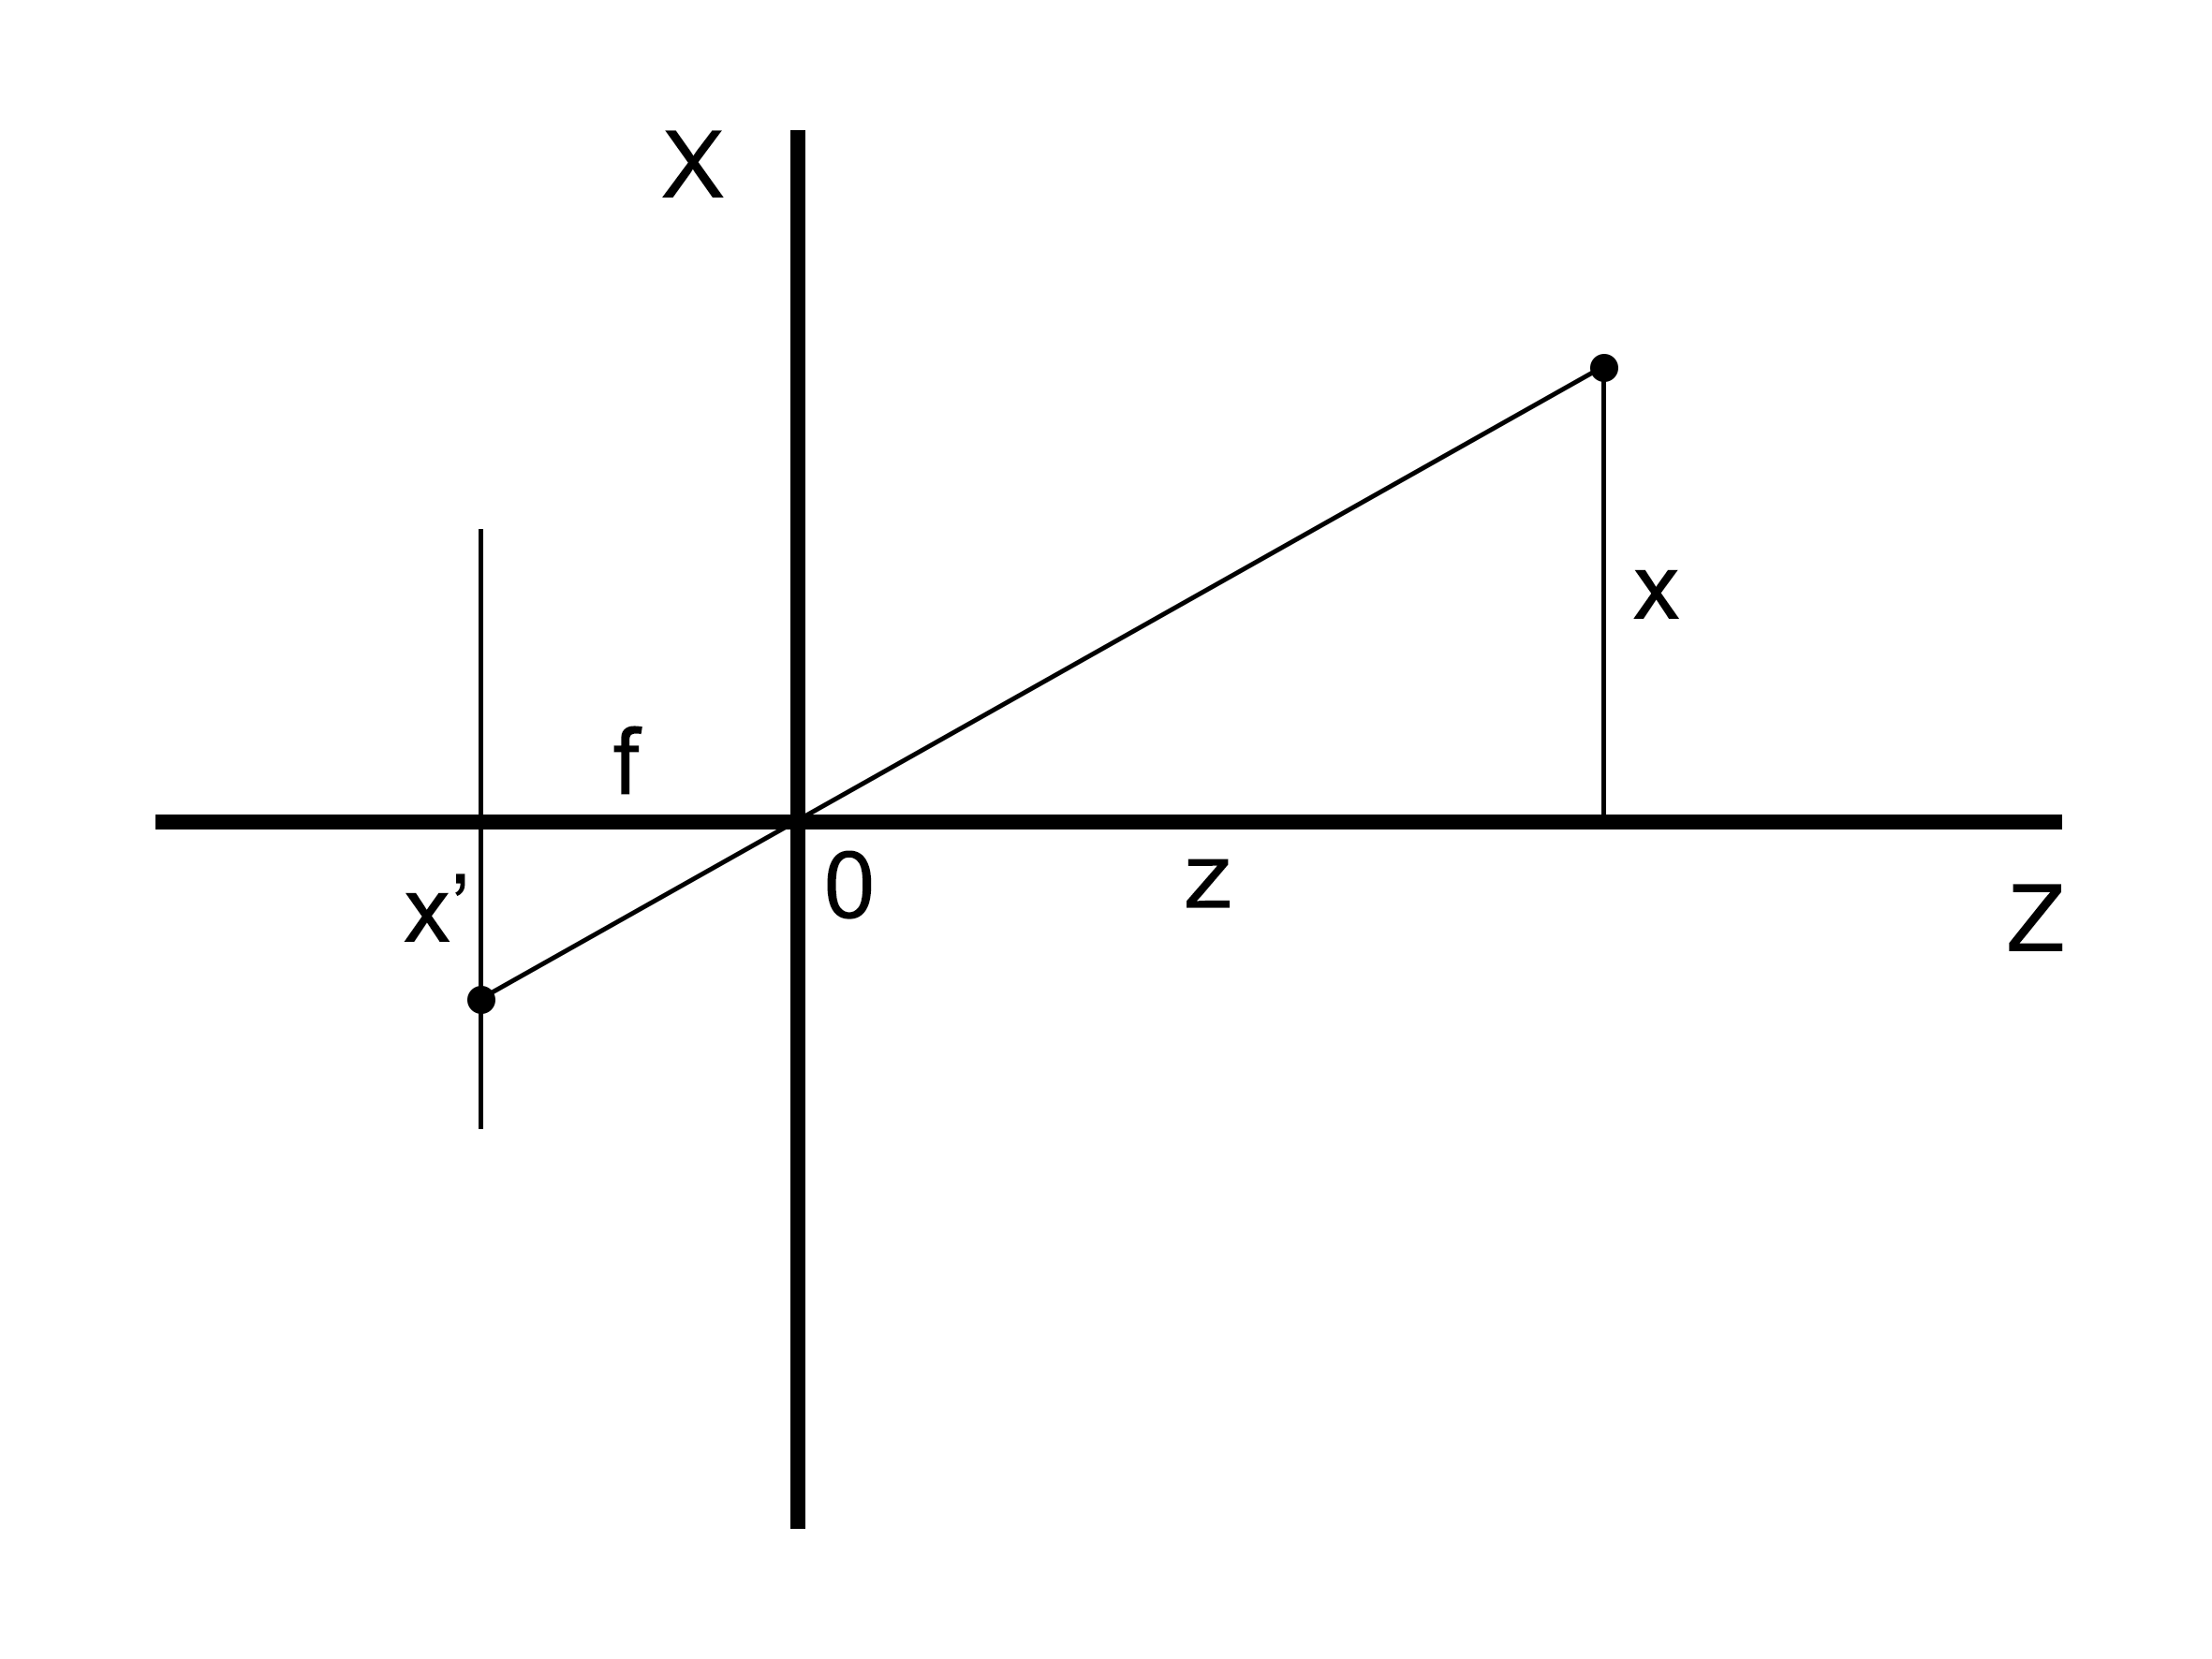
\includegraphics[width=\textwidth,height=\textheight,keepaspectratio]{similar_triangles_1.png}
\caption{Točka v svetu (desno) se preslika na slikovno ploskev (levo).}
\label{similar1}
\end{figure}

Izhodišče predstavlja luknjico kamere. Višina točke v svetu je predstavljena z $x$, oddaljenost od kamere pa z $z$. Točka na sliki je označena z $x’$, goriščna razdalja pa s $f$. Točka v svetu se preko luknjice (koordinatnega izhodišča) preslika na slikovno ploskev. Vse točke v svetu so na slikovni ploskvi obrnjene za 180°, kar pa kamere samodejno popravijo, ko vrnejo sliko. Za lažje računanje pa lahko to ugotovitev uporabimo za vpeljavo navidezne slikovne ploskve. 

\begin{figure}[H]
\centering
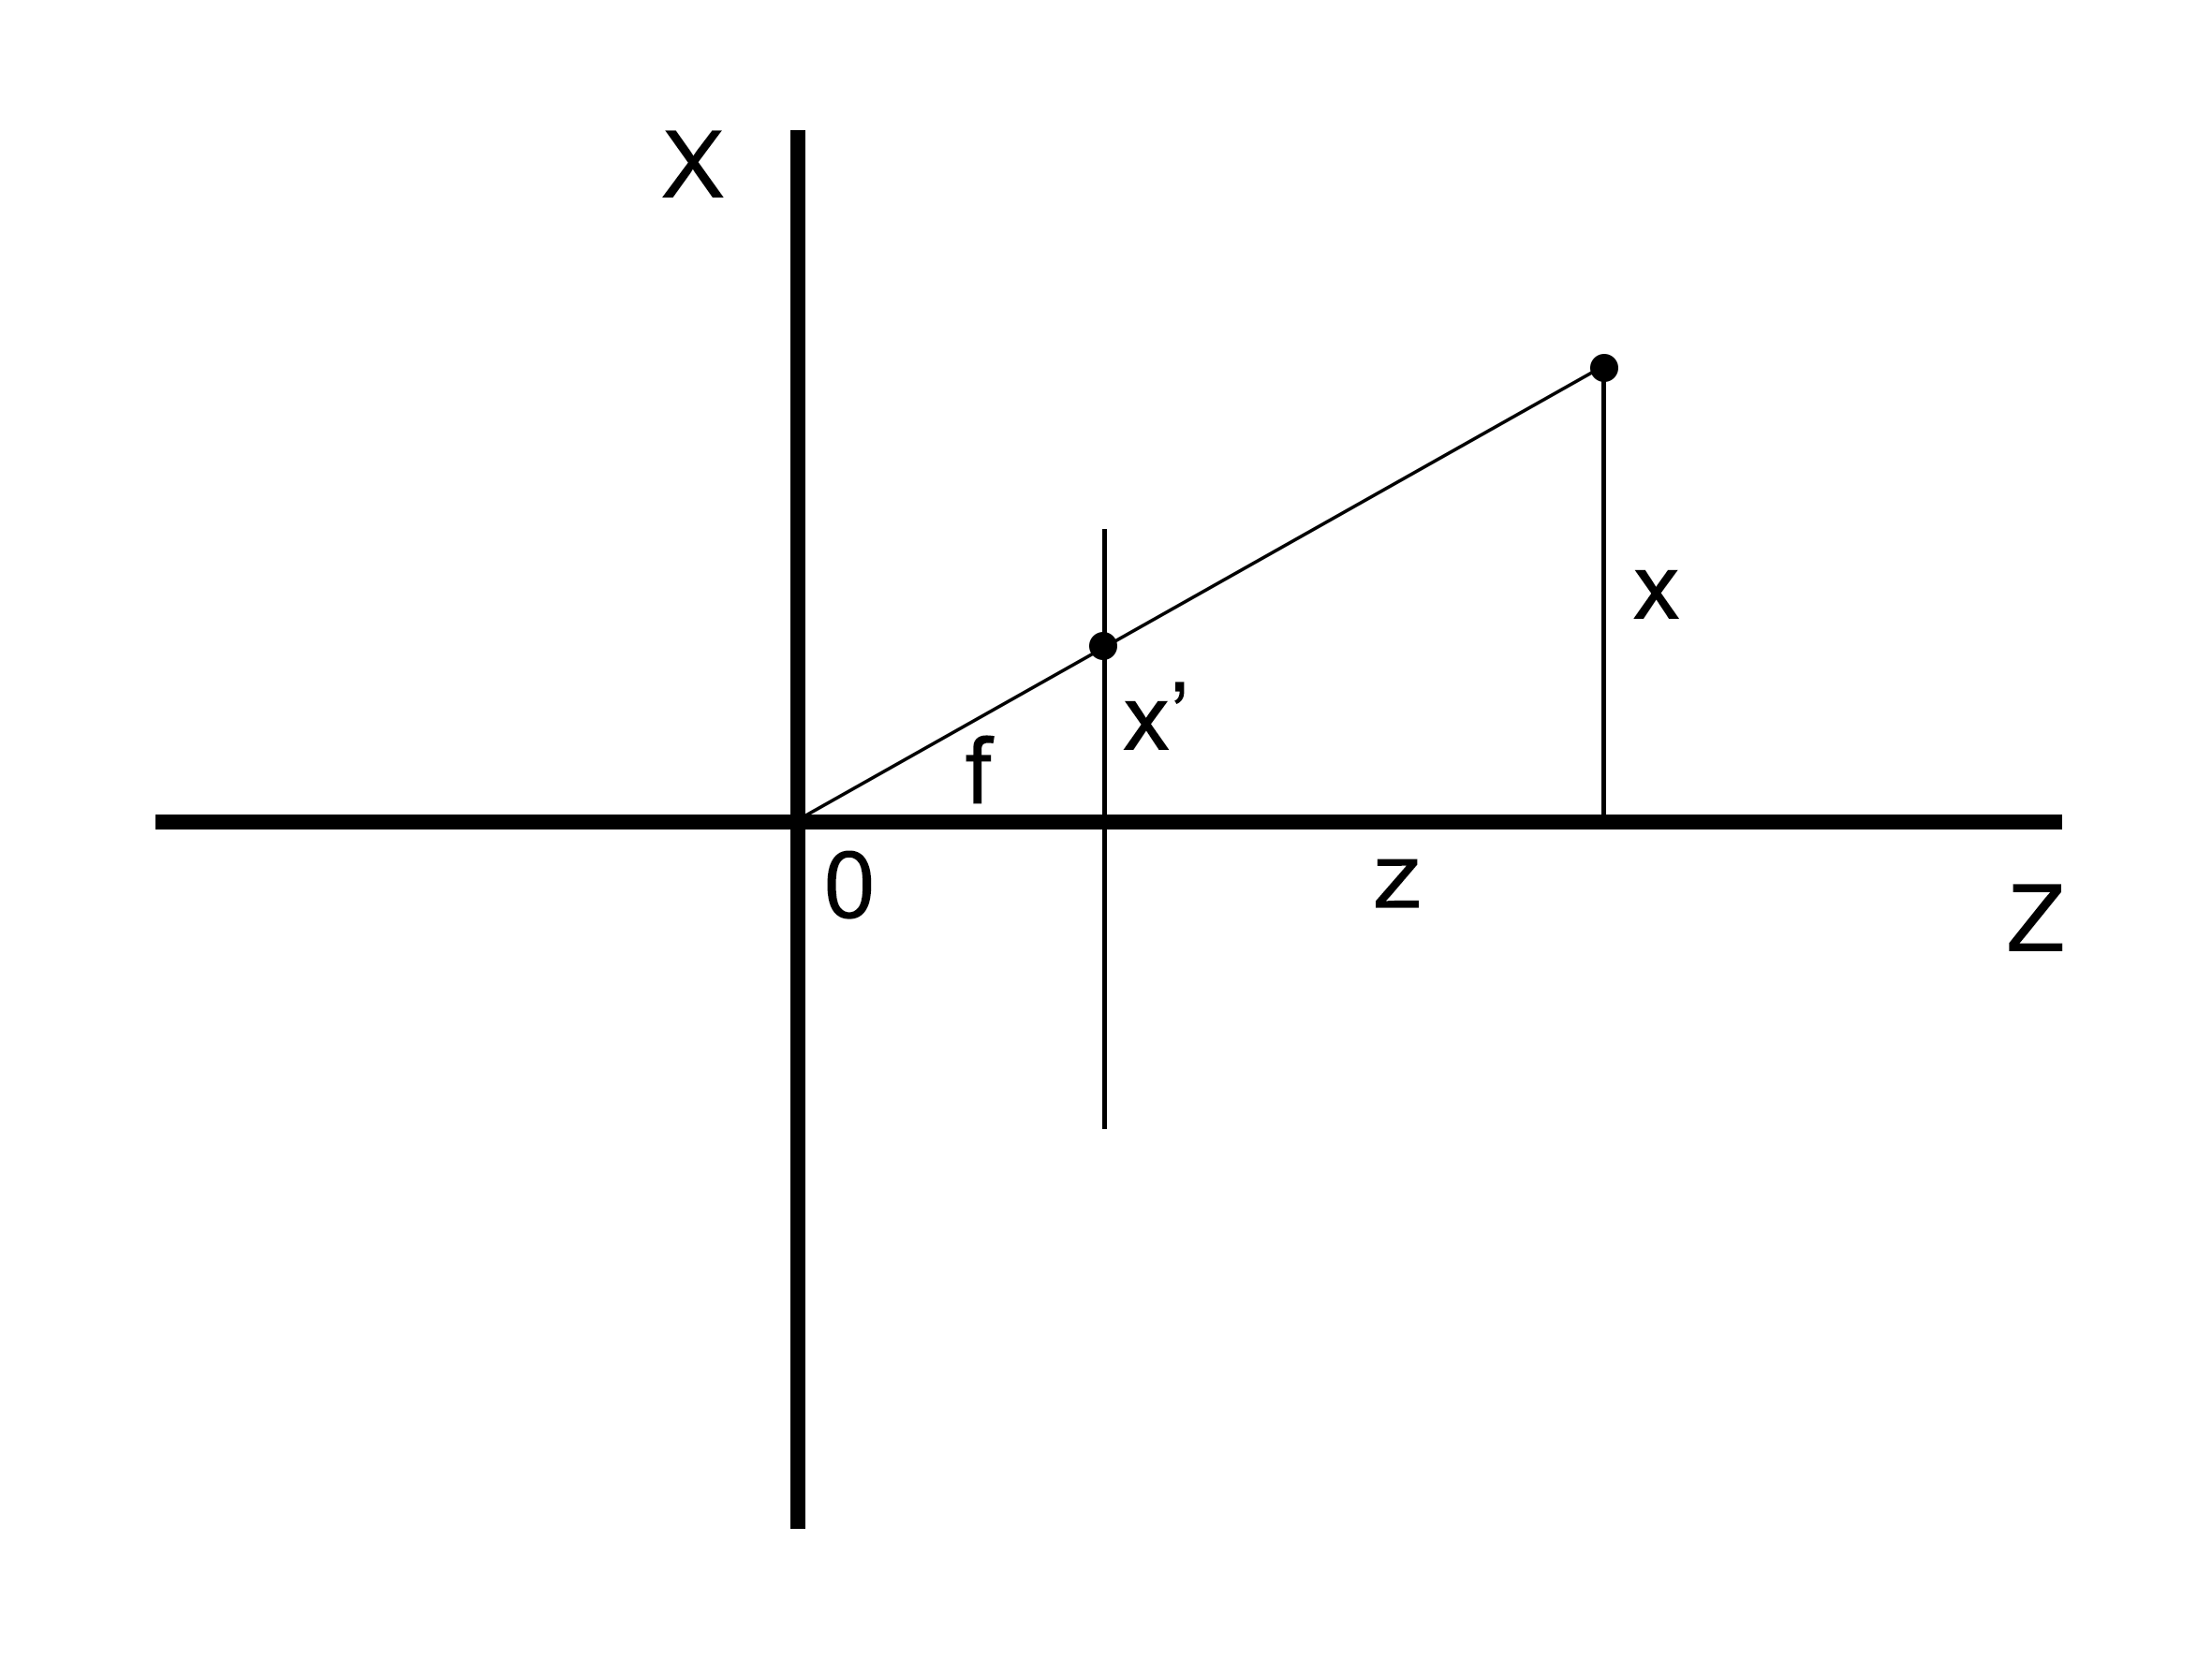
\includegraphics[width=\textwidth,height=\textheight,keepaspectratio]{similar_triangles_2.png}
\caption{Na sliki se jasno vidi dva podobna pravokotna trikotnika.}
\label{similar2}
\end{figure}

Hitro opazimo, da je preslikava iz sveta na sliko linearna operacija. Na sliki \ref{similar2} vidimo podobna pravokotna trikotnika, ki ju določa točka v svetu in točka na sliki. Vzpostavimo lahko relacijo,
\begin{align}
\frac{x'}{f} &= \frac{x}{z} \\
x' &= f * \frac{x}{z}
\end{align}
Če formulo posplošimo na obe koordinatni osi dobimo,
\begin{align}
\begin{bmatrix}
x' \\
y'
\end{bmatrix}
&= \frac{f}{z}
\begin{bmatrix}
x \\
y
\end{bmatrix}
\label{simplemodeleq}
\end{align}

Enačba \eqref{simplemodeleq} predstavlja najpreprostejši model kamere z luknjico. Ima seveda veliko pomanjkljivost, ki pa jih bomo postopoma odpravili. Enačbo \eqref{simplemodeleq} se da zapisati še preprosteje z uvedbo homogenih koordinat.
\begin{align}
\begin{bmatrix}
x' \\
y' \\
1
\end{bmatrix}
&\sim 
\begin{bmatrix}
f*x \\
f*y \\
z
\end{bmatrix}
\end{align}

Točka v homogenih koordinatah ni enolično določena z vrednostmi točke saj za homogeno točko $x$ velja $x \sim \lambda x$, kjer $\lambda \neq 0$. Homogeno točko preslikamo nazaj v evklidski prostor tako, da vse koordinate delimo z zadnjo vrednostjo točke. 

Pri predstavitvi digitalnih slik je izhodišče običajno v levem zgornjem kotu. Zgornji model pa predpostavlja izhodišče v sredini slike. V model moramo vpeljati dve konstanti $u$ in $v$, ki bosta prestavili izhodišče koordinatnega sistema slike. To se lahko kompaktno zapiše kot množenje točke v svetu z matriko.
\begin{align}
\begin{bmatrix}
x' \\
y' \\
1
\end{bmatrix}
&\sim
\begin{bmatrix}
f & 0 & u \\
0 & f & v \\
0 & 0 & 1
\end{bmatrix}
\begin{bmatrix}
x \\
y \\
z
\end{bmatrix}
\end{align}

Zgornji model predpostavlja, da so pike na senzorju kamere kvadratne. Dandanes je za veliko kamer to tudi res. Ker pa se da pravokotne ali celo poševne pike enostavno vključiti v obstoječi model, bomo to naredili.
\begin{align}
\begin{bmatrix}
x' \\
y' \\
1
\end{bmatrix}
&\sim
\begin{bmatrix}
f*m_x & s & u \\
0 & f*m_y & v \\
0 & 0 & 1
\end{bmatrix}
\begin{bmatrix}
x \\
y \\
z
\end{bmatrix}
\label{internaleq}
\end{align}

Enačba \eqref{internaleq} predstavlja notranji model kamere. Goriščna razdalja je označena s $f$, $m_x$ in $m_y$ predstavljata velikost, $s$ pa poševnost pike, $u$ in $v$ pa določata principalno točko. Vektor $[x \ y \ z]^T$ določa točko v svetu, $[x' \ y' \ 1]^T$ pa kam se ta točka preslika na sliko.

Slike iz kamer so lahko tudi popačene. Obstajata dve vrsti popačenosti, ki ju prej opisani model ne more modelirati. To sta radialna in tangencialna popačenost. Radialno popačenost povzroči oblika leče in poznamo dve glavni različici:
\begin{enumerate}
\itemsep0em
\item sodčasto, ki spominja na obliko soda in
\item blazinasto, ki spominja na obliko blazine
\end{enumerate}
Obstaja še kombinacija obeh, ki pa se imenuje brkato popačenje (ker spominja na obliko brk).

\begin{figure}[H]
\centering
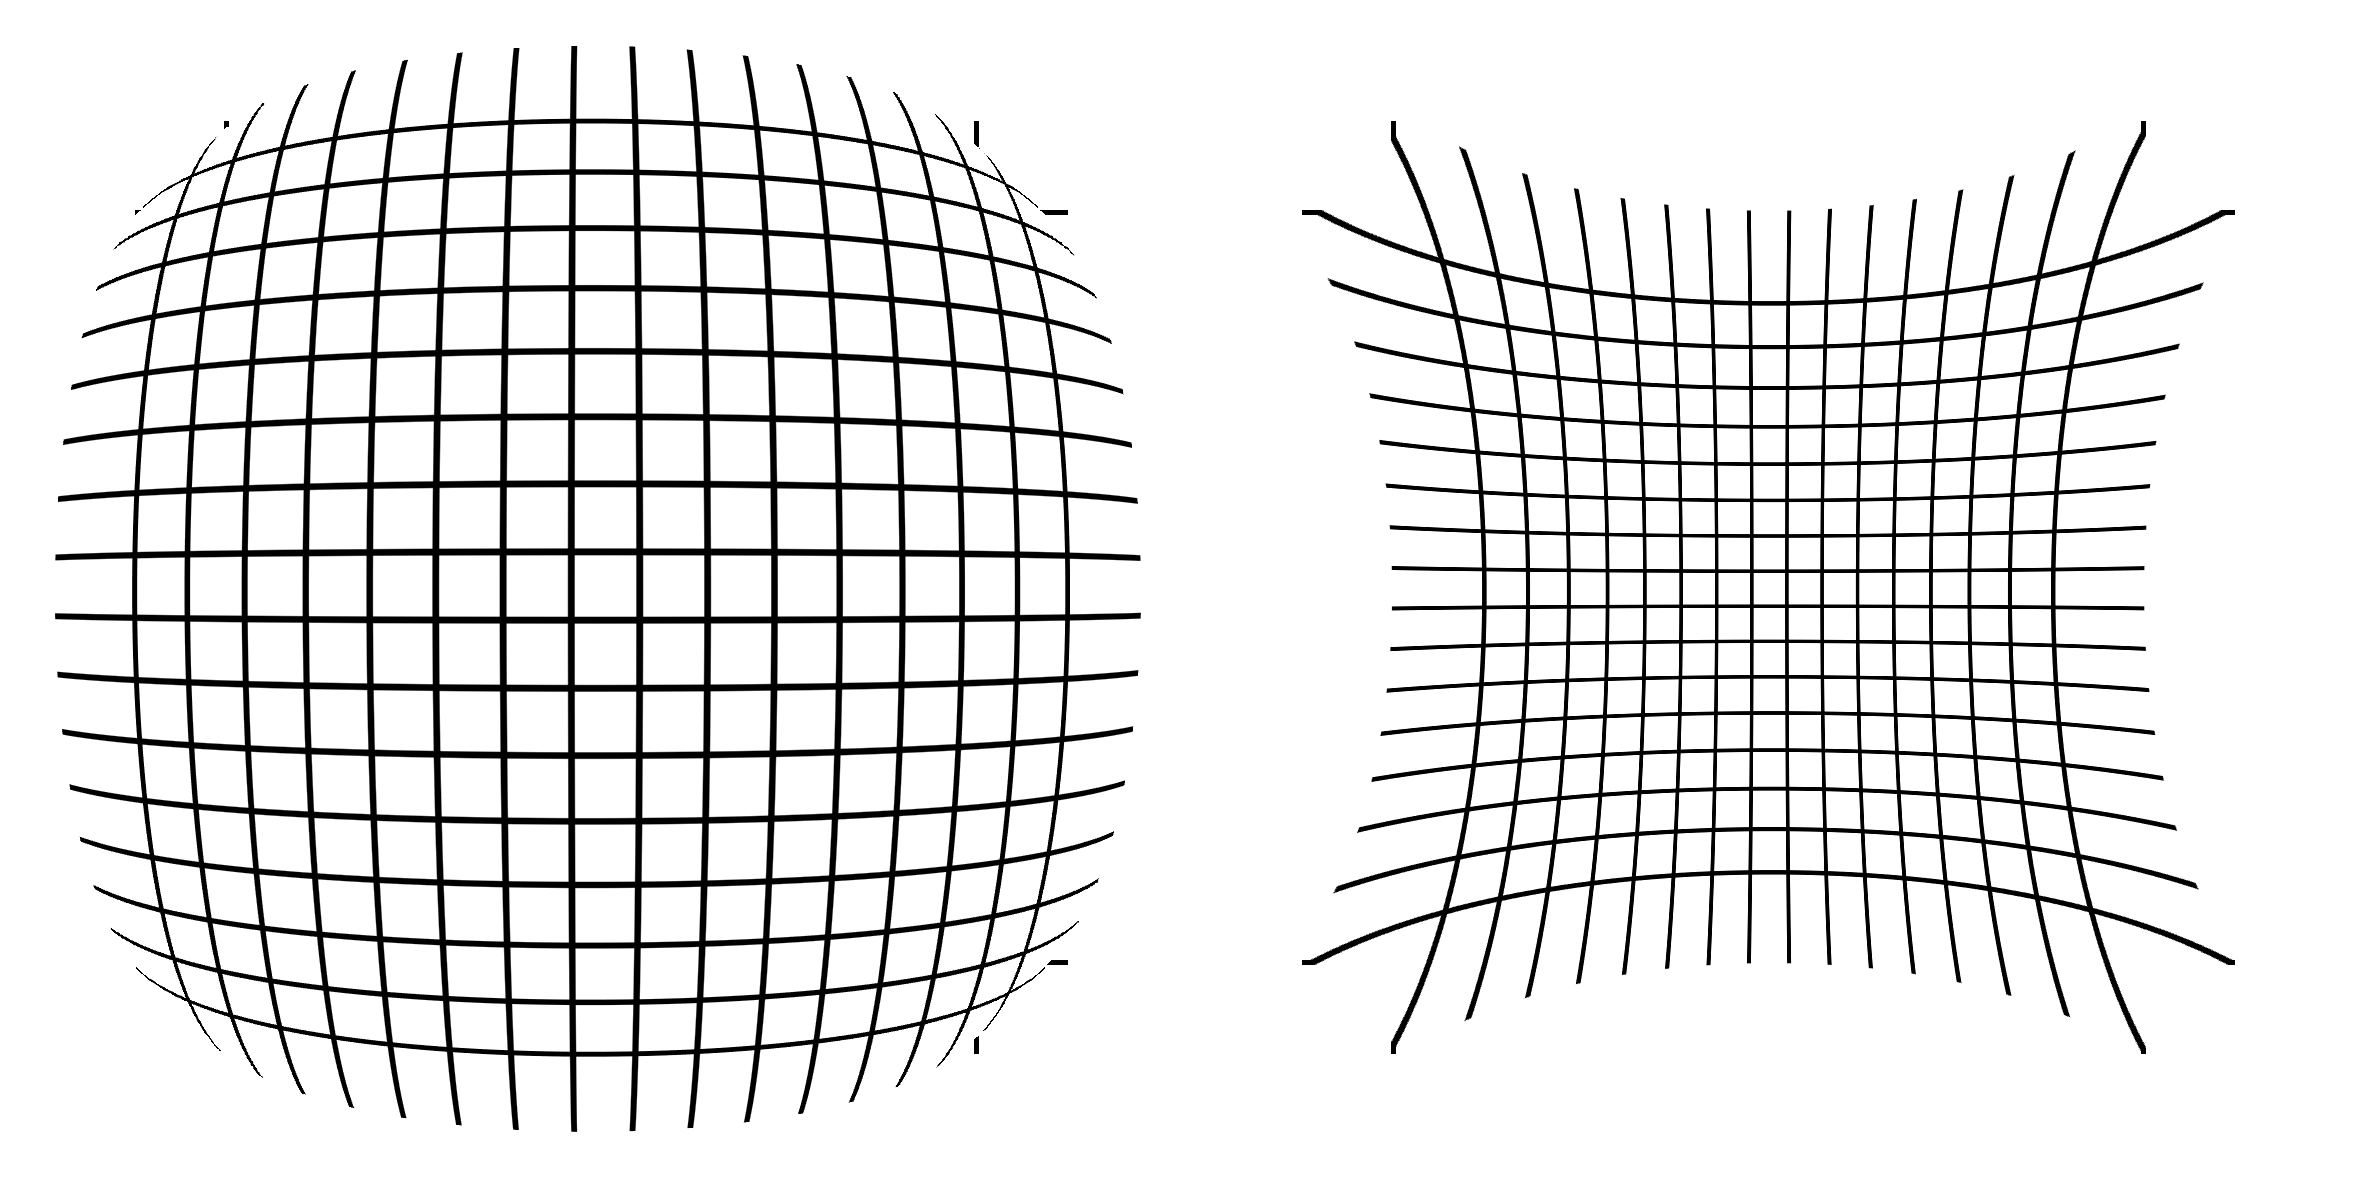
\includegraphics[width=\textwidth,height=\textheight,keepaspectratio]{distorsion.png}
\caption{Sodčasta popačenost (levo), blazinasta popačenost (desno).}
\end{figure}

Moč radialne popačenosti slikovne točke je odvisna od razdalje do principalne točke. Modeliramo jo lahko z vsotami polinomov sodih stopenj. Za večino radialnih popačenj zadoščata že dva koeficienta. 
\begin{align}
\label{radialdisteq}
r &= \sqrt{x^2 + y^2} \\ 
x_{popaceno} &= x * (1 + k_1*r^2 + k_2*r^4 + k_3*r^6 + \dots) \\
y_{popaceno} &= y * (1 + k_1*r^2 + k_2*r^4 + k_3*r^6 + \dots)
\end{align}

Druga popačenost, ki jo poznamo pa je tangencialna in nastane zaradi slabe poravnanosti leč in senzorja.

\begin{figure}[H]
\centering
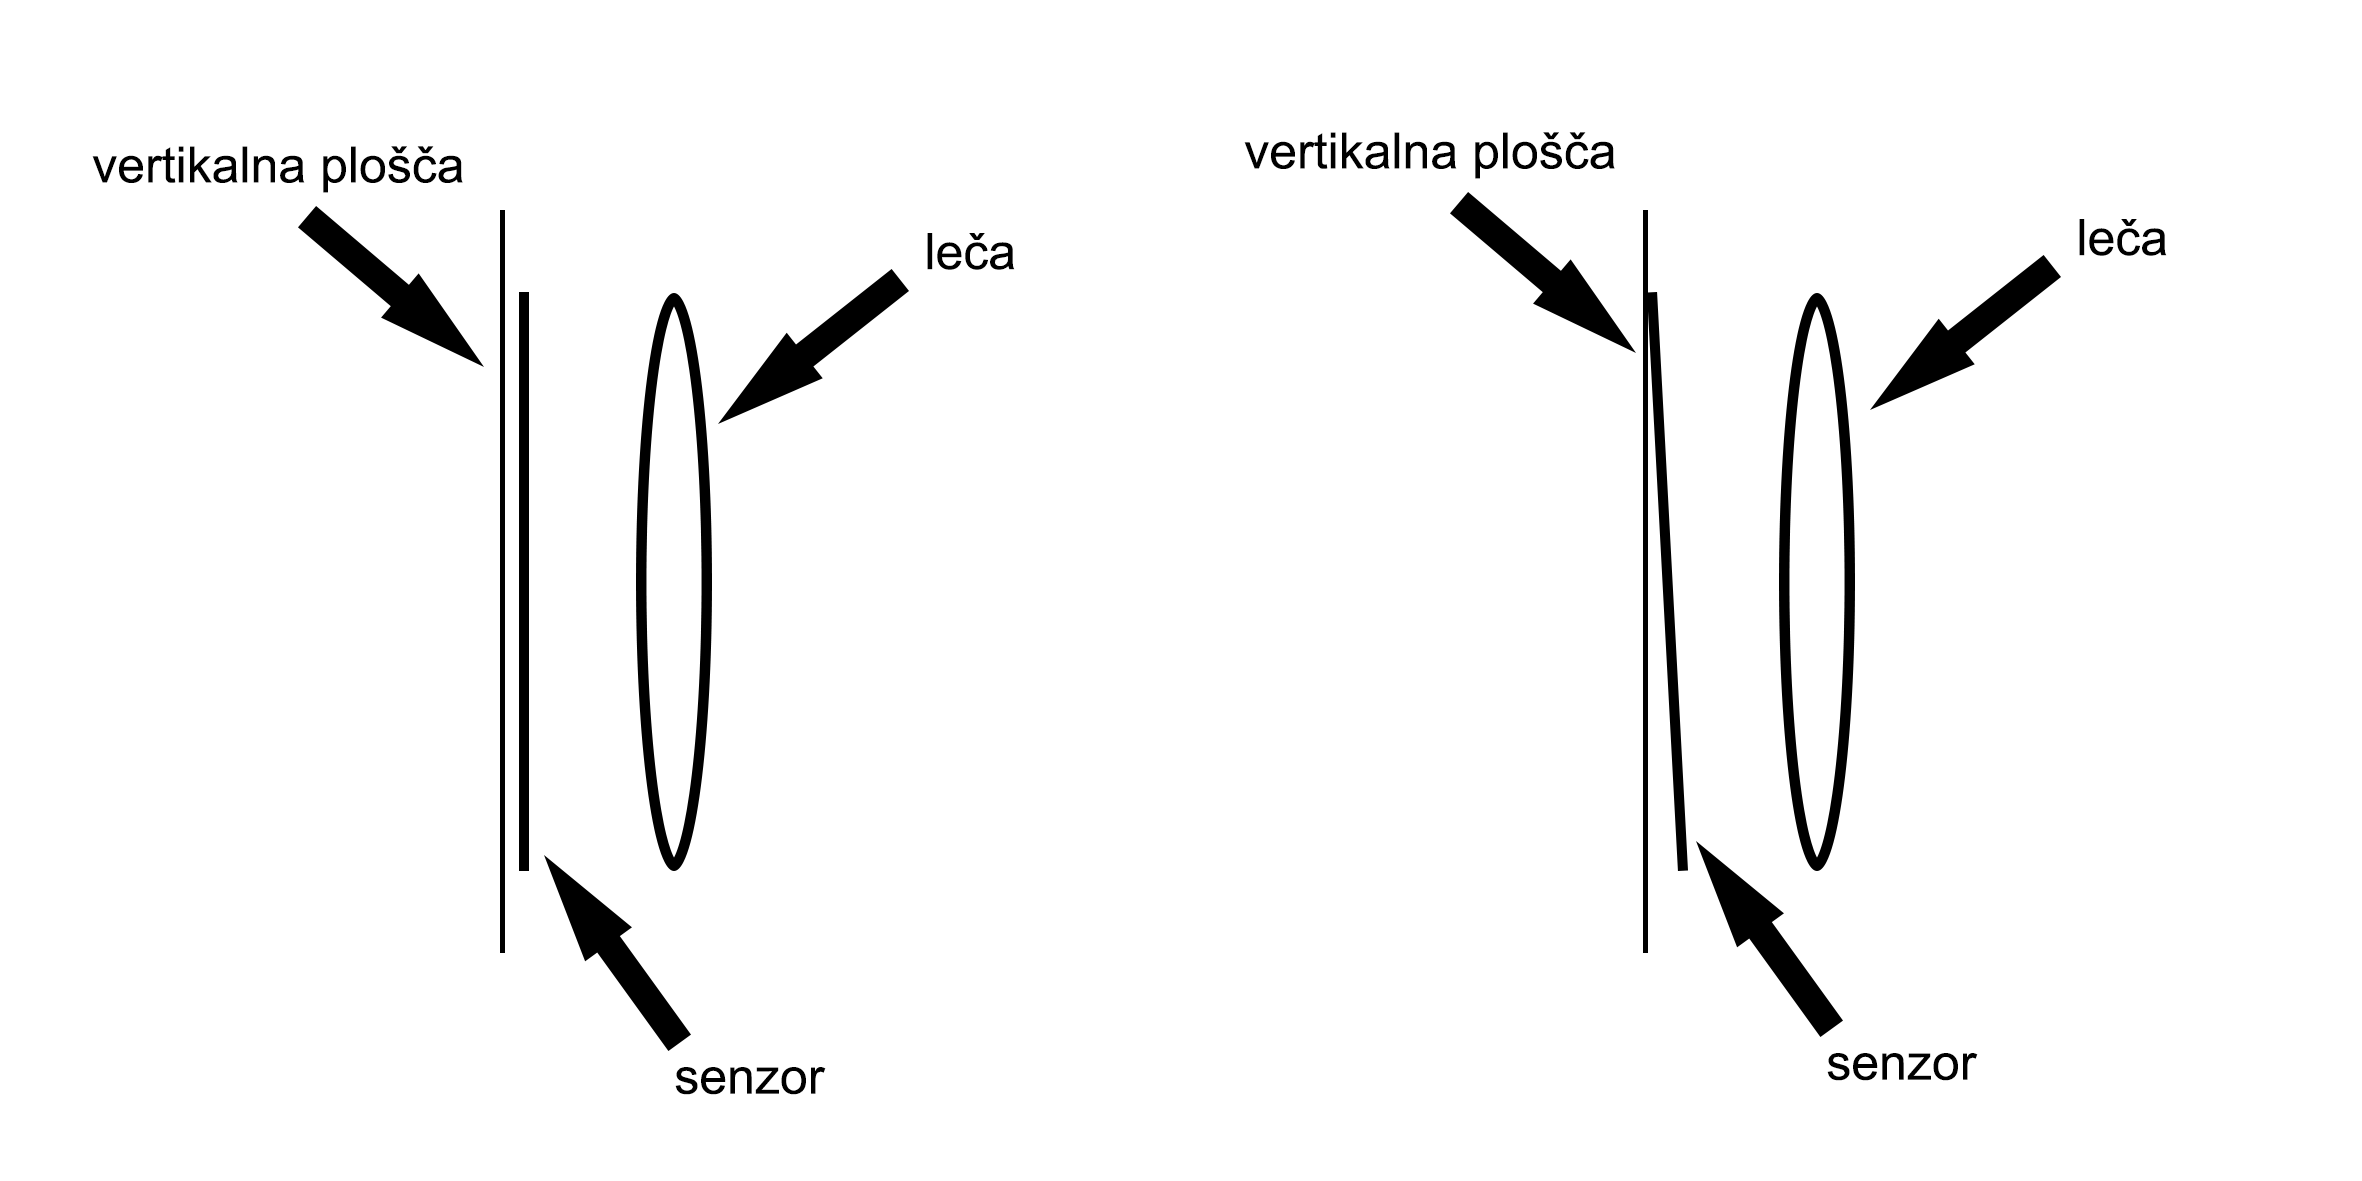
\includegraphics[width=\textwidth,height=\textheight,keepaspectratio]{tangential.png}
\caption{Senzor in leča sta vzporedna zato do tangencialne popačenosti v tem primeru ne pride (levo).}
\end{figure}

Modeliramo jo lahko kot,
\begin{align}
\label{tangentialdisteq}
r &= \sqrt{x^2 + y^2} \\ 
x_{popaceno} &= x + (2 * p_1 * x * y + p_2 * (r^2 + 2 * x^2)) \\
y_{popaceno} &= y + (p_1 * (r^2 + 2*y^2) + 2 * p_2 * x * y)
\end{align}

Če povzamemo, notranje parametre kamere določa matrika A in koeficienti popačenja. Koeficiente se lahko predstavi z vektorjem $\vec{r}$, ki določa radialno popačenost in z vektorjem $\vec{t}$, ki določa tangencialno popačenost.
\begin{align*}
A &= 
\begin{bmatrix}
f*m_x & s & u \\
0 & f*m_y & v \\
0 & 0 & 1
\end{bmatrix} \\
\vec{r} &= [k_1 \ k_2 \ k_3 \dots] \\
\vec{t} &= [p_1 \ p_2]
\end{align*}

\subsection{Zunanji parametri}
Do sedaj smo predpostavljali, da je koordinatno izhodišče sveta sama kamera. Uporabno bi bilo, če bi lahko poljubno določili koordinatni sistem sveta in vanj postavili kamere. Ravno temu so namenjeni zunanji parametri kamere. Med različnimi koordinatnimi sistemi lahko enolično prehajamo z rotacijo in translacijo. Če napišem malo drugače: iz enega koordinatnega sistema lahko dobimo kateri koli drug koordinatni sistem (z enakim št. dimenzij) tako, da izhodišči poravnamo s translacijo in nato rotiramo osi, da sovpadajo. 

Rotacijo v treh dimenzijah lahko predstavimo z množenjem matrike $R$ velikosti $3 \times 3$. Translacija pa je vsota točke v svetu $\vec{X}$ in translacijskega vektorja $\vec{T}$.
\begin{equation}
\vec{X}_{premaknjen} = R * \vec{X} + \vec{T} = 
\begin{bmatrix}
r_{11} & r_{12} & r_{13} \\
r_{21} & r_{22} & r_{23} \\
r_{31} & r_{32} & r_{33}
\end{bmatrix}
* 
\begin{bmatrix}
x \\
y \\
z 
\end{bmatrix}
+
\begin{bmatrix}
x_t \\
y_t \\
z_t 
\end{bmatrix}
\label{coordeq}
\end{equation}

Izkaže se, da če točko v svetu predstavimo s homogenimi koordinatami, lahko enačbo \eqref{coordeq} zapišemo kot množenje matrike $[R | \vec{T}]$ z vektorjem $\vec{X}$.
\begin{equation}
\vec{X}_{premaknjen} = [R|\vec{T}] * \vec{X} = 
\begin{bmatrix}
r_{11} & r_{12} & r_{13} & x_t\\
r_{21} & r_{22} & r_{23} & y_t\\
r_{31} & r_{32} & r_{33} & z_t
\end{bmatrix}
* 
\begin{bmatrix}
x \\
y \\
z \\
1
\end{bmatrix}
\label{coordeq}
\end{equation}
Zavedati se moramo, da rotacijska matrika $R$ in translacijski vektor $\vec{T}$ ne predstavljata rotacijo in pozicijo kamere v svetu, ampak rotacijo in pozicijo sveta relativno na kamero. Rotacijo kamere lahko dobimo z $R^{-1} = R^T$, pozicijo v svetu pa z $-R^{-1} * \vec{T} = -R^T * \vec{T}$.

\subsection{Model kamere}

Model \eqref{internaleq} lahko dopolnimo z zunanjimi parametri ter tako dobimo popolen model kamere.
\begin{align}
\label{totalmodel}
\vec{X}' &\sim A * [R | \vec{T}] * \vec{X} \\
\begin{bmatrix}
x' \\
y' \\
1
\end{bmatrix}
&\sim
\begin{bmatrix}
f*m_x & s & u \\
0 & f*m_y & v \\
0 & 0 & 1
\end{bmatrix}
*
\begin{bmatrix}
r_{11} & r_{12} & r_{13} & x_t\\
r_{21} & r_{22} & r_{23} & y_t\\
r_{31} & r_{32} & r_{33} & z_t
\end{bmatrix}
*
\begin{bmatrix}
x \\
y \\
z \\
1
\end{bmatrix} \\
\vec{r} &= [k_1 \ k_2 \ k_3 \dots] \\
\vec{t} &= [p_1 \ p_2]
\end{align}

\section{Ocenjevanje parametrov}
V poglavju \ref{parametri} je opisan model kamere. Kamero določajo razni parametri, ki pa so za vsako kamero različni. V tem poglavju bom opisal kako oceniti posamezne parametre kamere, da bo model postal uporaben.

\subsection{Ocenjevanje notranjih parametrov}
Za ocenjevanje notranjih parametrov kamere obstaja veliko algoritmov, ki pa se razlikujejo po hitrosti, težavnosti in natančnosti. Dve popularni metodi sta Tsaijev kalibracijski algoritem \cite{horn2000tsai} in Zhangova fleksibilna tehnika za kalibracijo kamer \cite{zhang2000flexible}. Sam sem za ocenjevanje notranjih parametrov uporabil MATLAB-ovo kalibracijsko orodje, ki uporablja variacijo Zhangove tehnike. Več o samem postopku kalibracije je opisano v poglavju \ref{camcalsec}. 

\subsection{Ocenjevanje zunanjih parametrov}\label{externalparamssection}
Zunanji parametri kamere določajo kje v prostoru se kamera nahaja. Zgoraj omenjena Zhangova metoda poleg notranjih vrne tudi zunanje parametre, ki pa za namen diplomskega dela niso uporabni, saj bi morali kamere kalibrirati z vsaj eno sliko ploskve, ki jo v celoti vidijo vse kamere. Sistem mora delovati tudi, če imajo kamere minimalno ali celo ničelno prekrivanje vidnega polja. V nadaljevanju bom opisal teoretično podlago metode, ki sem jo uporabil za ocenjevanje zunanjih parametrov. Doseči želimo, da kameram določimo skupen koordinatni sistem sveta.

Metoda predpostavlja, da imamo za neko kamero že izračunane notranje parametre. Za oceno zunanjih parametrov je dovolj le ena slika iz kamere, ki pa ne sme biti popačena. Najprej je torej potrebno popačeno sliko popraviti. Enačbe \eqref{radialdisteq} in \eqref{tangentialdisteq} določajo neposredno preslikavo med popačenimi in nepopačenimi točkami. 
\begin{equation}
\vec{X}' \sim A * [R | \vec{T}] * \vec{X}
\label{cammodeleq}
\end{equation}

Zunanje parametre določa rotacijska matrika $R$ in translacijski vektor $\vec{T}$, kar je v zgornji enačbi kompaktno predstavljeno z matriko $[R | \vec{T}]$. Za oceno teh parametrov moramo poznati notranje parametre $A$, točko v svetu $X$ in njeno projekcijo na sliko $X'$. Matriko $[R | \vec{T}]$ lahko ocenimo z metodo DLT (\emph{ang. Direct Linear Transformation}). Ker računamo s homogenimi koordinatami, sta si leva in desna stran enačbe enaka do poljubnega neničelnega faktorja $\lambda$. Enačbo \eqref{cammodeleq} lahko zapišemo z
\begin{equation}
\lambda * \vec{X}' = A * [R | \vec{T}] * \vec{X}
\label{lambdaeq}
\end{equation}

Z eno znano točko (na sliki in v svetu) dobimo 3 enačbe, vendar pa je ena linearna kombinacija drugih dveh, zato nam pri ocenjevanju zunanjih parametrov ne pomaga. Oceniti moramo torej 12 neznank (ker je $[R | \vec{T}]$ matrika velika $3 \times 4$), z eno točko pa dobimo 2 neodvisni enačbi, kar pomeni, da potrebujemo najmanj 6 točk za katere poznamo svetovne koordinate in njihove projekcije na sliko. Dobimo torej sistem enačb,

\begin{align*}
\lambda_1 * \vec{X}_1' &= A * [R | \vec{T}] * \vec{X_1} \\
\lambda_2 * \vec{X}_2' &= A * [R | \vec{T}] * \vec{X_2} \\
\lambda_3 * \vec{X}_3' &= A * [R | \vec{T}] * \vec{X_3} \\
&\vdots
\end{align*}

Problem predstavljajo neničelni faktorji na levi strani enačb, saj jih ne poznamo in so odvisni od zunanjih parametrov kamere. Metoda DLT reši ravno tak sistem enačb. Leva stran je pravzaprav 3-dimenzionalni vektor za katerega vemo, da je vedno enak nič, če ga vektorsko pomnožimo s samim seboj. Vektorsko množenje pa lahko predstavimo z matričnim množenjem.
\begin{align}
\vec{a} &= 
\begin{bmatrix}
a_1 \\
a_2 \\
a_3
\end{bmatrix} \\
\vec{a} \times \vec{a} = [\vec{a}]_{\times} * \vec{a} &= 
\begin{bmatrix}
0 & -a_3 & a_2 \\
a_3 & 0 & -a_1 \\
-a_2 & a_1 & 0
\end{bmatrix}
* \begin{bmatrix}
a_1 \\
a_2 \\
a_3
\end{bmatrix} = 0
\end{align}

Obe strani enačbe \eqref{lambdaeq} lahko pomnožimo z leve z $[\vec{X}']_{\times}$.
\begin{align}
\lambda * [\vec{X}']_{\times} * \vec{X}' &= [\vec{X}']_{\times} * A * [R | \vec{T}] * \vec{X} \\
0 &= [\vec{X}']_{\times} * A * [R | \vec{T}] * \vec{X}
\end{align}

S tem korakom smo se znebili neznanega parametra $\lambda$, vendar iz take oblike enačbe težko najdemo rešitev sistema. Za lažjo izpeljavo bomo enačbo \eqref{lambdaeq} z leve pomnožili z inverzom matrike $A$.

\begin{align}
\label{uvw}
A^{-1} * \vec{X}' &=
\begin{bmatrix}
u \\
v \\
w
\end{bmatrix} \\
[A^{-1} * \vec{X}']_{\times} &=
\begin{bmatrix}
0 & -w & v \\
w & 0 & -u \\
-v & u & 0
\end{bmatrix} \\[5ex]
\lambda * A^{-1} * \vec{X}' &= [R | \vec{T}] * \vec{X} \\
0 &= [A^{-1} * \vec{X}']_{\times} * [R | \vec{T}] * \vec{X}\\
0 &= 
\begin{bmatrix}
0 & -w & v \\
w & 0 & -u \\
-v & u & 0
\end{bmatrix}
*
\begin{bmatrix}
p_1 & p_2 & p_3 & p_4 \\
p_5 & p_6 & p_7 & p_8 \\
p_9 & p_{10} & p_{11} & p_{12}
\end{bmatrix}
*
\begin{bmatrix}
x \\
y \\
z \\
1
\end{bmatrix} \\
0 &= 
\begin{bmatrix}
x(-wp_5 + vp_9) + y(-wp_6 + vp_{10}) + z(-wp_7 + vp_{11}) + (-wp_8 + vp_{12}) \\
x(wp_1 - up_9) + y(wp_2 - up_{10}) + z(wp_3 - up_{11}) + (wp_4 - up_{12}) \\
x(-vp_1 + up_5) + y(-vp_2 + up_6) + z(-vp_3 + up_7) + (-vp_4 + up_8)
\end{bmatrix}
\label{longeq}
\end{align}

\setcounter{MaxMatrixCols}{20}
Sistem enačb \eqref{longeq} lahko zapišemo v obliki $B * \vec{p} = 0$, kjer
\begin{align}
\vec{p} &= [p_1 \ p_2 \ p_3 \ p_4 \ p_5 \ p_6 \ p_7 \ p_8 \ p_9 \ p_{10} \ p_{11} \ p_{12}]^T \\
B &=
\begin{bmatrix}
0 & 0 & 0 & 0 & -xw & -yw & -zw & -w & xv & yv & zv & v \\
xw & yw & zw & w & 0 & 0 & 0 & 0 & -xu & -yu & -zu & -u \\
-xv & -yv & -zv & -v & xu & yu & zu & u & 0 & 0 & 0 & 0
\end{bmatrix}
\label{bmatrix}
\end{align}

Zadnja vrstica v matriki $B$ je linearna kombinacija prvih dveh. Za vsak par točk (v svetu in na sliki) generiramo prvi dve vrstici matrike $B$ in vse vrstice združimo v skupno matriko $B$ velikosti $2n \times 12$, kjer je $n$ število parov točk. Sistem enačb lahko sedaj rešimo z razcepom na singularne vrednosti (\emph{ang. SVD - Singular Value Decomposition}). SVD razcepi matriko $B$ na $U \Sigma V^T$, kjer je $U$ matrika levih lastnih vektorjev, $\Sigma$ matrika singularnih vrednosti in $V$ matrika desnih lastnih vektorjev. Po definiciji za leve lastne vektorje matrike $B$ velja $B * \vec{v} = \lambda * \vec{v}$, kjer je $\lambda$ lastna vrednost. Če iz matrike $V$ vzamemo vektor, ki ustrza najmanjši lastni vrednosti v matriki $\Sigma$, smo tako dobili netrivialno rešitev, ki najbolje zadošča pogoju $B * \vec{p} = 0$. Rešitev je potrebno le še preoblikovati v $3 \times 4$ matriko zunanjih parametrov. V poglavju \ref{camcalsec} naslovim problem, ki nastane, če matrika $B$ nima ranga $12$, kar se zgodi, če ocenjujemo parametre s koplanarnimi točkami v prostoru.

\section{Triangulacija}

Iz modela \eqref{totalmodel} želimo oceniti $\vec{X}$. Uporabimo lahko podoben postopek kot pri ocenjevanju zunanjih parametrov.

\begin{align}
\lambda * \vec{X}' &= A * [R | \vec{T}] * \vec{X} \\
0 &= [\vec{X}']_{\times} * A * [R | \vec{T}] * \vec{X} \\
B &= [\vec{X}']_{\times} * A * [R | \vec{T}] \\
B * \vec{X} &= 0
\end{align}

Rang matrike B mora biti 4, saj ocenjujemo štiri parametre, ki določajo X. Ena točka na sliki nam poda 2 linearno neodvisni enačbi. Potrebujemo torej vsaj 2 različni točki iz dveh različnih slik, ki predstavljata projekcijo iste točke v prostoru na sliko. Sistem zopet rešimo z razcepom na singularne vrednosti kot smo to naredili v prejšnjem poglavju.

\section{Zaznavanje označevalnika}\label{markersection}

Pri zaznavanju označevalnika je potrebno sliko iz kamere segmentirati. Segmentacija je postopek ločevanja ozadja od objekta zanimanja. Označevalnik ima običajno izrazito drugačno barvo od okolice, zato da pri zaznavanju ne prihaja do dvoumnosti. Segmentacija ponavadi vrne binarno sliko, kjer je ozadje predstavljeno z vrednostjo 0, segmenti pa z vrednostjo 1. 

Segmentiramo lahko tako sivinsko kot barvno sliko. Za vsako točko v sliki se moramo odločiti ali pripada ozadju (0) ali segmentu (1). Če so vrednosti pik predstavljene z monotono naraščujočimi vrednostmi, lahko določimo prag, ki ločuje ozadje od segmenta. Spodaj je podana psevdo koda segmentacije.
\begin{lstlisting}
I //sivinska slika
w // sirina slike
h // visina slika
T //prag
for i = 1...h
    for j = 1...w
        if I[i][j] > T
            I[i][j] = 1
        else
            I[i][j] = 0
\end{lstlisting}

Pri segmentiranju barvnih slik se je potrebno odločiti za primeren barvni model. Primarno so slike zapisane v rdečem, zelenem in modrem kanalu (model RGB). Običajno je bolj primeren model HSV ali HSL, saj H (ton, \emph{ang. hue}) komponenta določa barvo neodvisno od njene intenzitete in nasičenosti. Slednja modela sta pri segmentaciji bolj robustna, ker sprememba svetlobe ne vpliva toliko na spremembo tonskega kanala.

Izbira barvnega modela in praga je za vsak primer specifična. Včasih je bolje uporabiti model RGB npr. v primeru, če ima označevalnik izrazito barvo ne glede na osvetljitev.

Iz segmentirane slike moramo izračunati središče zaznanega objekta (če je prisoten na sliki). To lahko storimo s slikovnimi momenti. Prostorski momenti na sivinski sliki I so definirani kot,
\begin{equation}
M_{ij} = \sum_x \sum_y x^i * y^j * I(x, y)
\end{equation}

Poznamo še centralne momente, ki pa so definirani kot,
\begin{align}
\bar{x} &= \frac{M_{10}}{M_{00}} \\
\bar{y} &= \frac{M_{01}}{M_{00}} \\
\mu_{ij} &= \sum_x \sum_y (x - \bar{x})^i * (y - \bar{y})^j * I(x, y)
\end{align}

Masno središče je predstavljeno z $\bar{x}$ in $\bar{y}$. Moment $M_{00}$ je enak površini segmenta, $M_{10}$ ter $M_{01}$ pa sta vsoti vrednosti po $x$ in $y$ koordinatah.

\chapter{Implementacija}

\section{Strojna oprema}

\subsection{Računalnik}
Vsa obdelava podatkov se odvija na enem prenosnem računalniku. Zajemanje slik poteka sočasno v ločenih procesih. Računalnik ima dve fizični procesni jedri in štiri niti. V lokalno omrežje je povezan preko brezžične povezave. 

\begin{table}[H]
\centering
\begin{tabular}{| r | l |}
\hline
CPE & Intel i7-4510U 2.6 GHz \\
Pomnilnik & 8 GB \\
Št. jeder/niti & 2 / 4 \\
Arhitektura & 64-bit \\
OS & Windows 8.1 Pro \\
\hline
\end{tabular}
\caption{Specifikacije računalnika.}
\end{table}

\subsection{Kamere}
Uporabil sem štiri Axis 215 PTZ omrežne kamere. To so varnostne IP kamere namenjene primarno nadzoru okolja. Kamere so povezane v zvezdišče na omrežju ethernet, zvezdišče pa je povezano z brezžičnim usmerjevalnikom.  Kamere so zmožne v realnem času preko lokalnega omrežja posredovati do 30 slik na sekundo pri ločljivosti $704 \times 576$. Vseeno pa varnostne kamere niso namenjene za sinhronizirano zajemanje slik in ne podpirajo skupnega prožilca. Največja ločljivost je $704 \times 576$, kar je relativno malo za pozicioniranje objekta v $7,5 \times 7,5 \times 3 \ m^3$ velikem prostoru.
\begin{figure}[H]
\centering
\includegraphics[width=\textwidth,height=\textheight,keepaspectratio]{axis_215_ptz.png}
\caption{Axis 215 PTZ kamera.}
\end{figure}

\begin{table}[H]
\centering
\begin{tabular}{| r | l |}
\hline
Tip kamere & varnostna IP \\
Hitrost zajemanja & 30 FPS \\
Formati pretoka & MPEG-4, MJPEG \\
Največja ločljivost & 704 $\times$ 576 \\
Optična povečava & 12$\times$ \\
Digitalna povečava & 4$\times$ \\
Povezava z omrežjem & ethernet \\
Leča & 3,8 - 46 mm \\
\hline
\end{tabular}
\caption{Specifikacije Axis 215 PTZ.}
\end{table}

Axis kamere imajo CGI (\emph{ang. Common Gateway Interface}) vmesnik, ki omogoča nadzor funkcionalnosti preko protokola HTTP (\emph{ang. Hypertext Transfer Protocol}). Vsak model kamere podpira različen nabor ukazov, katerih spisek lahko dobimo z GET zahtevkom na naslov:
\begin{center}
\texttt{http://<ip-kamere>/axis-cgi/com/ptz.cgi?info=1}
\end{center}
Vsi ukazi pa so podani kot parameter v zahtevku.
\begin{center}
\texttt{http://<ip-kamere>/axis-cgi/com/ptz.cgi?<ukaz>=<vrednost>}
\end{center}
Spodaj je prikazan izpis ukaza \texttt{info=1} na Axis 215 PTZ kameri.
\begin{lstlisting}
Available commands
:
{camera=[n]}
whoami=yes
center=[x],[y]
   imagewidth=[n]
   imageheight=[n]
move={ home | up | down | left | right | upleft | upright | downleft | downright | stop }
pan=[abspos]
tilt=[abspos]
zoom=[n]
focus=[n]
rpan=[offset]
rtilt=[offset]
rzoom=[offset]
rfocus=[offset]
brightness=[offset]
rbrightness=[offset]
autofocus={ on | off }
ircutfilter={ on | off | auto }
backlight={ on | off }
continuouspantiltmove=[x-speed],[y-speed]
continuouszoommove=[speed]
continuousfocusmove=[speed]
auxiliary=[function]
setserverpresetname=[name]
setserverpresetno=[n]
removeserverpresetname=[name]
gotoserverpresetname=[name]
gotoserverpresetno=[n]
barcoord=[x],[y]
   panbar=[length],{ horizontal | vertical }
   tiltbar=[length],{ horizontal | vertical }
   zoombar=[length],{ horizontal | vertical }
   focusbar=[length],{ horizontal | vertical }
   irisbar=[length],{ horizontal | vertical }
   brightnessbar=[length],{ horizontal | vertical }
speed=[n]
query={ speed | position | presetposcam | presetposall }
\end{lstlisting}

%\vspace{2ex}
\subsection{Označevalnik}
Označevalnik je v osnovi oranžna žogica za namizni tenis. Da pa bi sprememba svetlobe čim manj vplivala na natančnost zazanavanja označevalnika, sem v žogico vgradil modro svetlečo diodo (\emph{LED - Light Emitting Diode}) in stikalo. S pritiskom na stikalo prižgemo označevalnik, da ga kamere lahko zaznajo. Na slikah kamer je žogica izrazito rumene barve.

\begin{figure}[H]
\centering
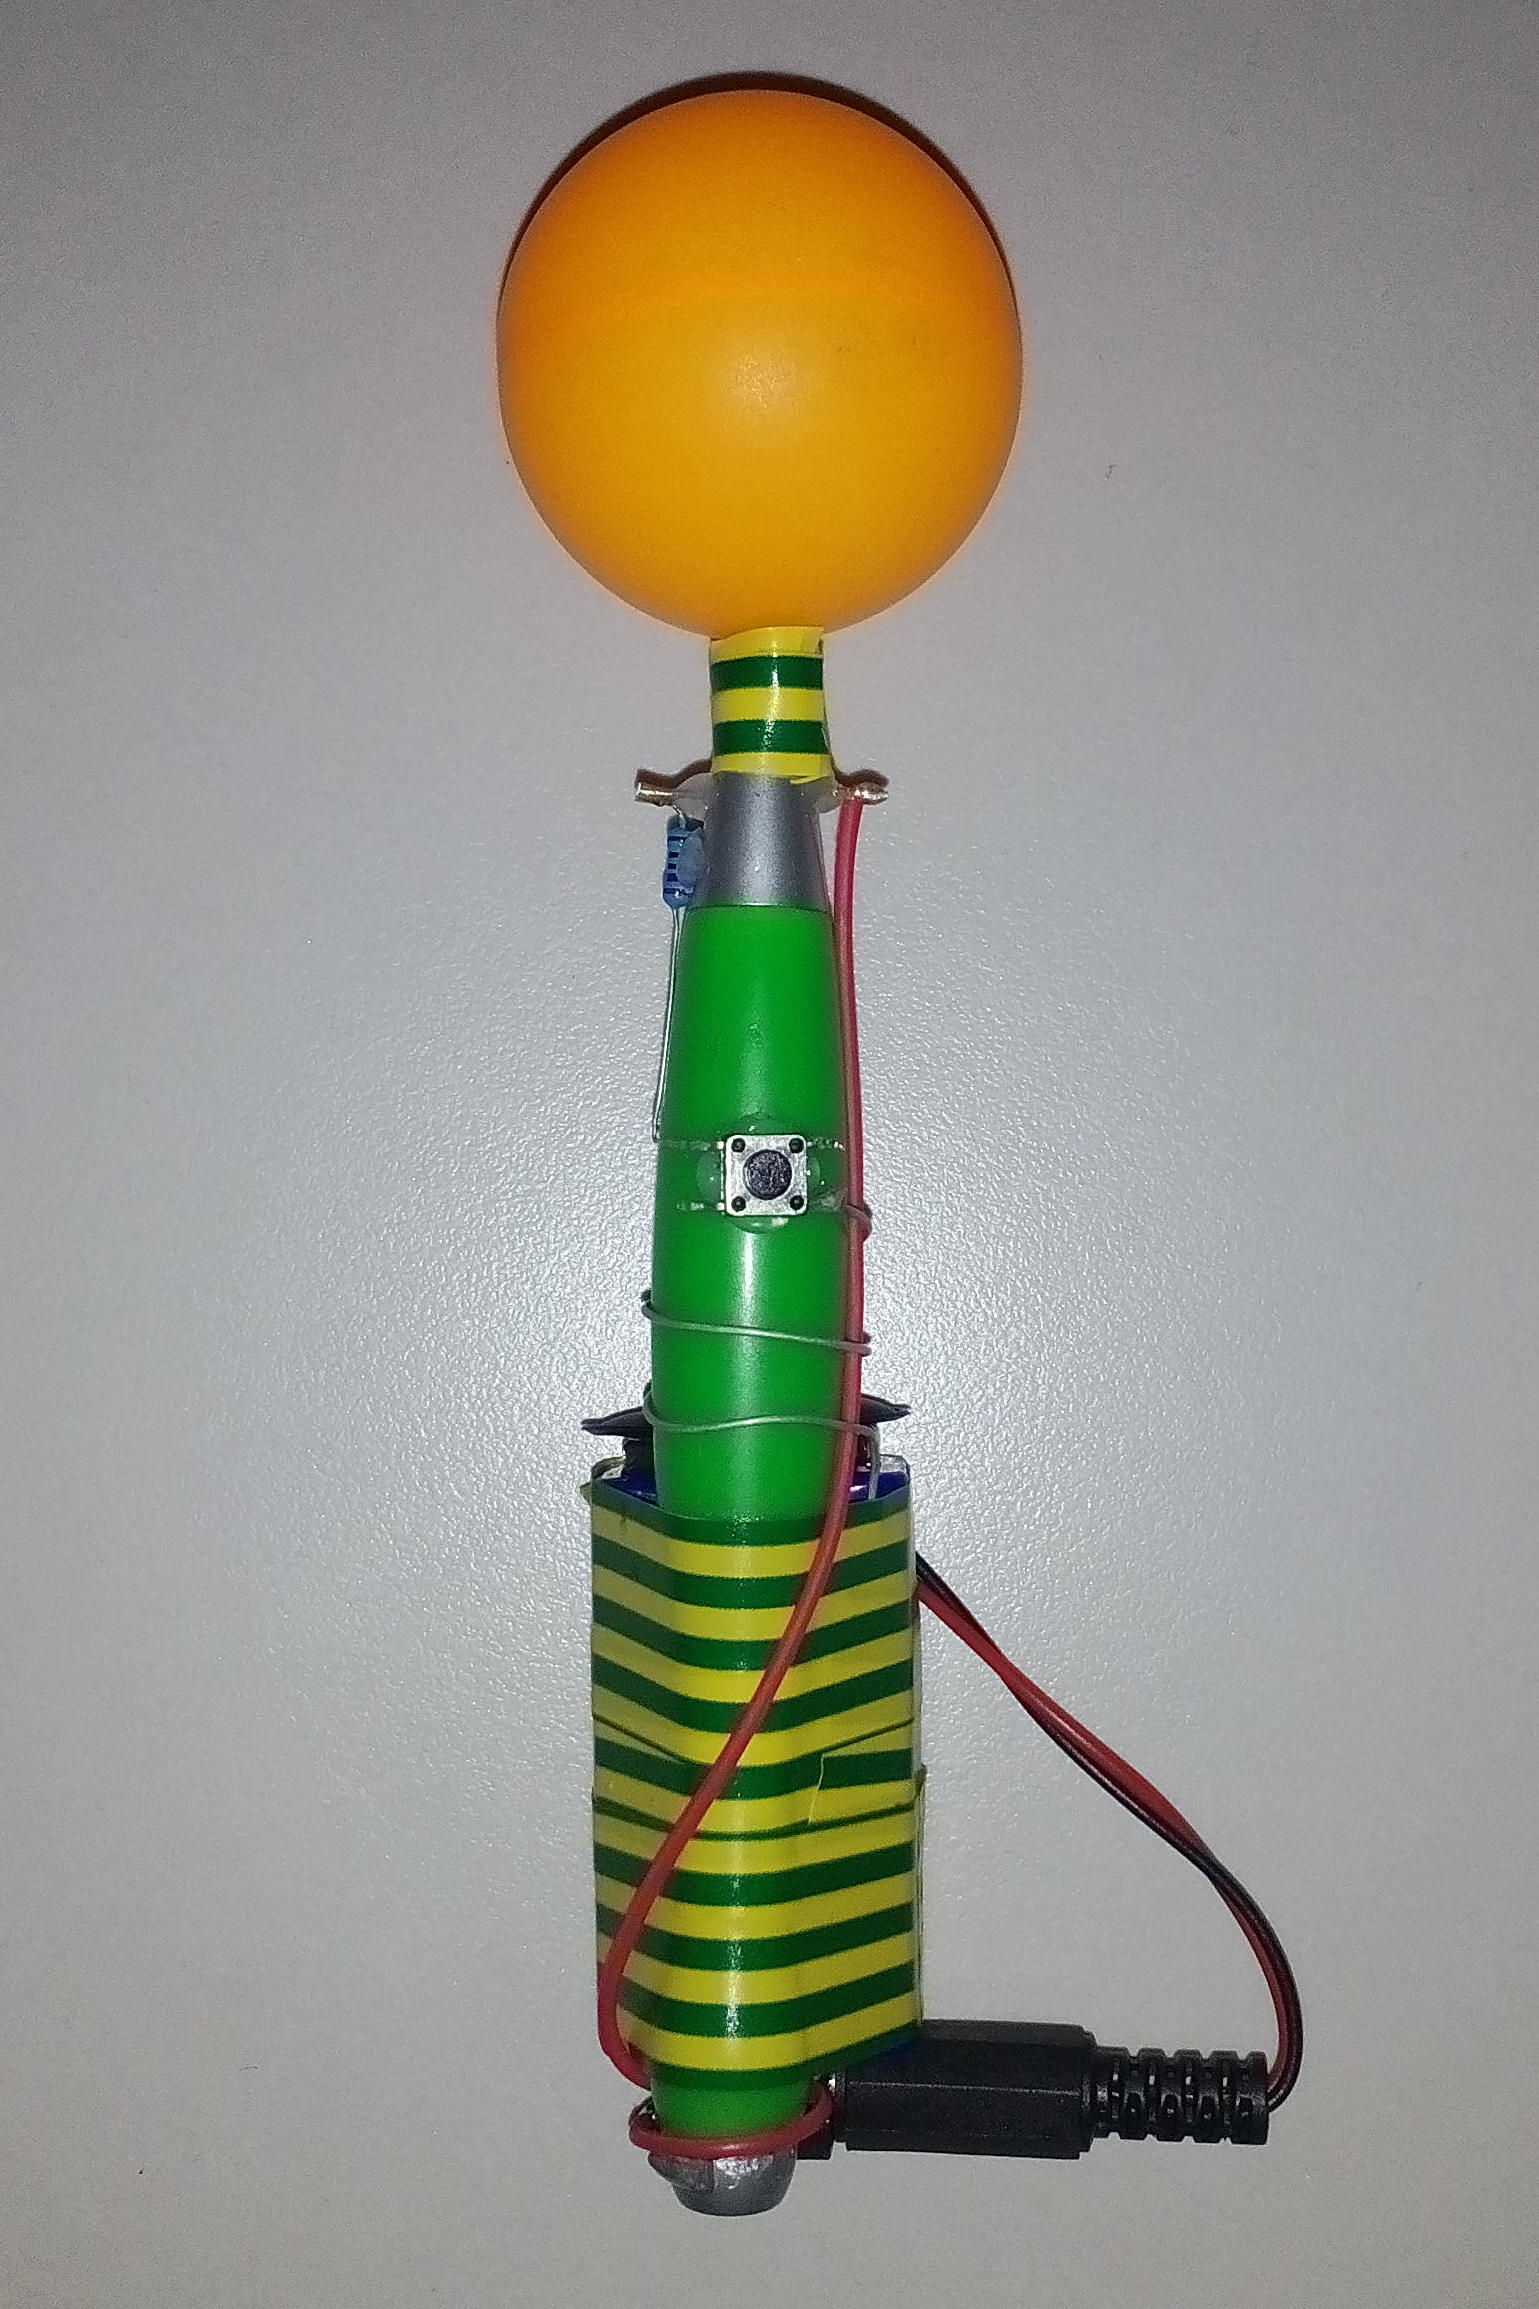
\includegraphics[scale=0.4]{marker_off.png}
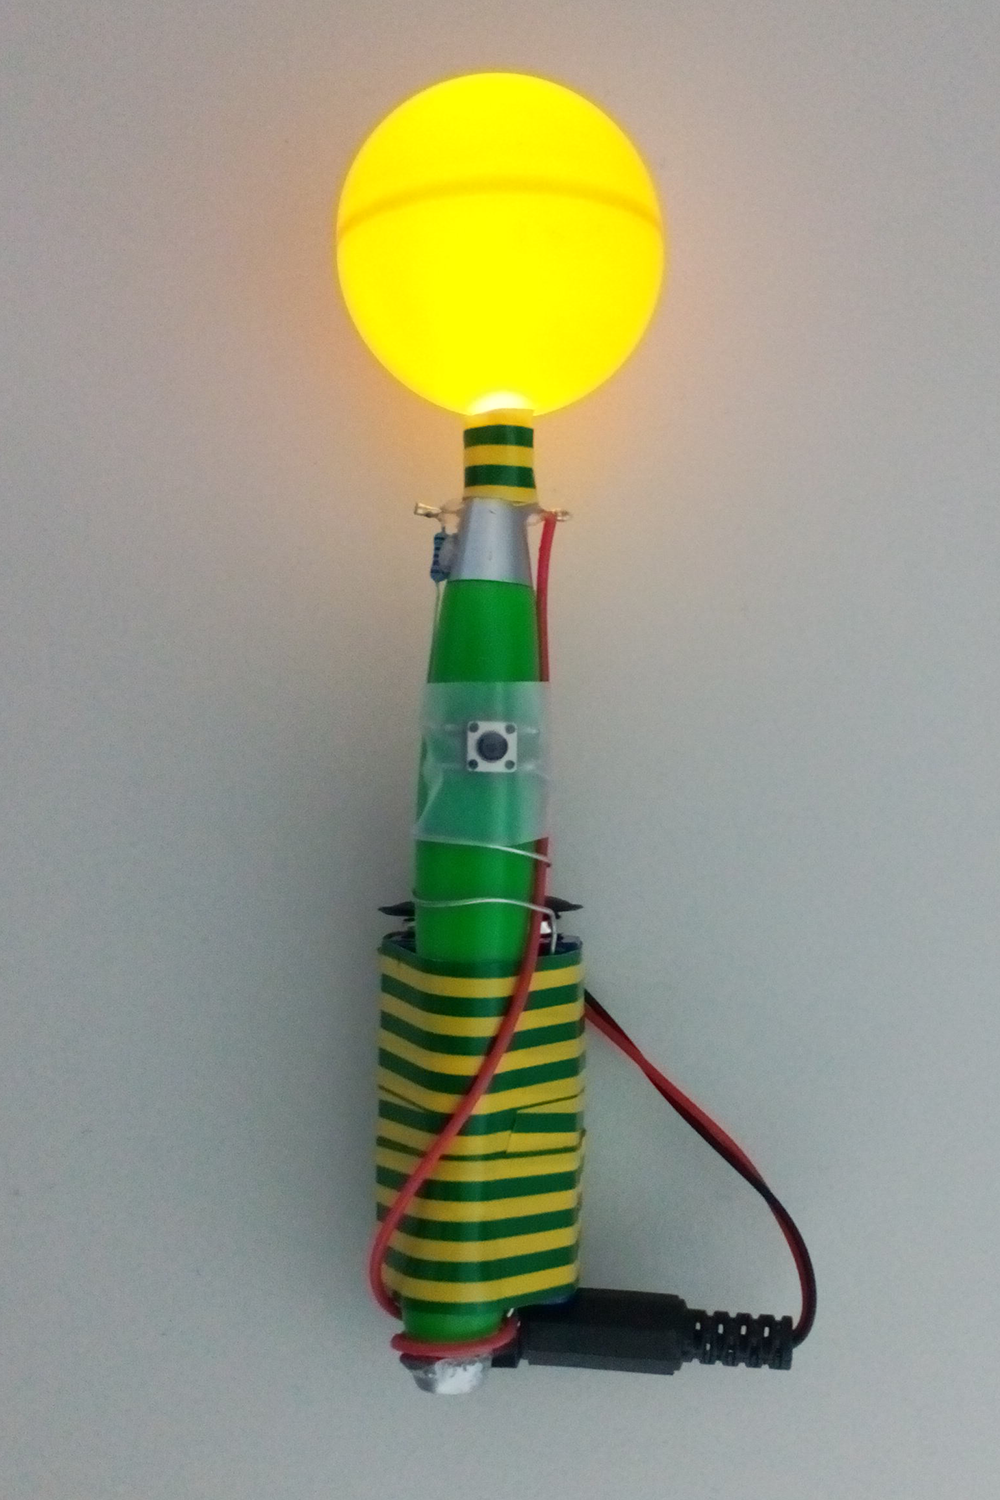
\includegraphics[scale=0.4]{marker_on.png}
\caption{Ugasnjen označevalnik je oranžne barve (levo), prižgan pa izrazito rumene barve (desno).}
\end{figure}

\section{Programska oprema}
Z delom sem začel v programu MATLAB R2014a. MATLAB je visokonivojski programski jezik in razvojno okolje, ki je primarno namenjeno prototipiranju. Podpira računanje z visokonivojskimi strukturami kot so matrike in vektorji. V njem sem razvil konceptno rešitev, ki sem jo nato implementiral v drugi aplikaciji. 

Za zajemanje statičnih slik iz kamer sem uporabil Node.js v0.12.3. Node.js je JavaScript pogon z veliko različnimi moduli. Node.js arhitektura je po zasnovi asinhrona, kar pri vhodno/izhodnih operacijah močno pohitri sistem.

Za iskanje kamer v omrežju sem uporabil Axisov IPUtility, ki samodejno vrne IP naslove vseh kamer, ki so priključene v omrežje.

Za implementacijo glavnega sistema pa sem uporabil Python 2.7 s knjižnicami Numpy v1.9.2, SciPy v0.15.1 ter OpenCV v3.0.0. Morda se zdi Python za realnočasovni sistem slaba izbira, vendar je s pravilno uporabo knjižnic odlično orodje za hitri razvoj. Funkcije v knjižnicah so zaradi hitrosti implementirane v njižjenivojskih jezikih kot so C/C++. Knjižnica Numpy je namenjena računanju z matrikami, SciPy pa je njena razširitev. OpenCV (Open Computer Vision) pa je namenjen za probleme umetnega zaznavanja in pri svoji implementaciji uporablja strukture Numpy-ja. 
\section{Kalibracija kamer}\label{camcalsec}
\subsection{Ocenjevanje notranjih parametrov}
Za ocenjevanje notranjih parametrov sem uporabil MATLAB-ov kalibrator kamere. Za kalibracijo mu moramo podati slike šahovnice, ki so bile zajete s kamero, ki jo želimo kalibrirati. Širina šahovnice mora biti različna od višine, da lahko enolično določimo njeno orientacijo. 
\begin{figure}[H]
\centering
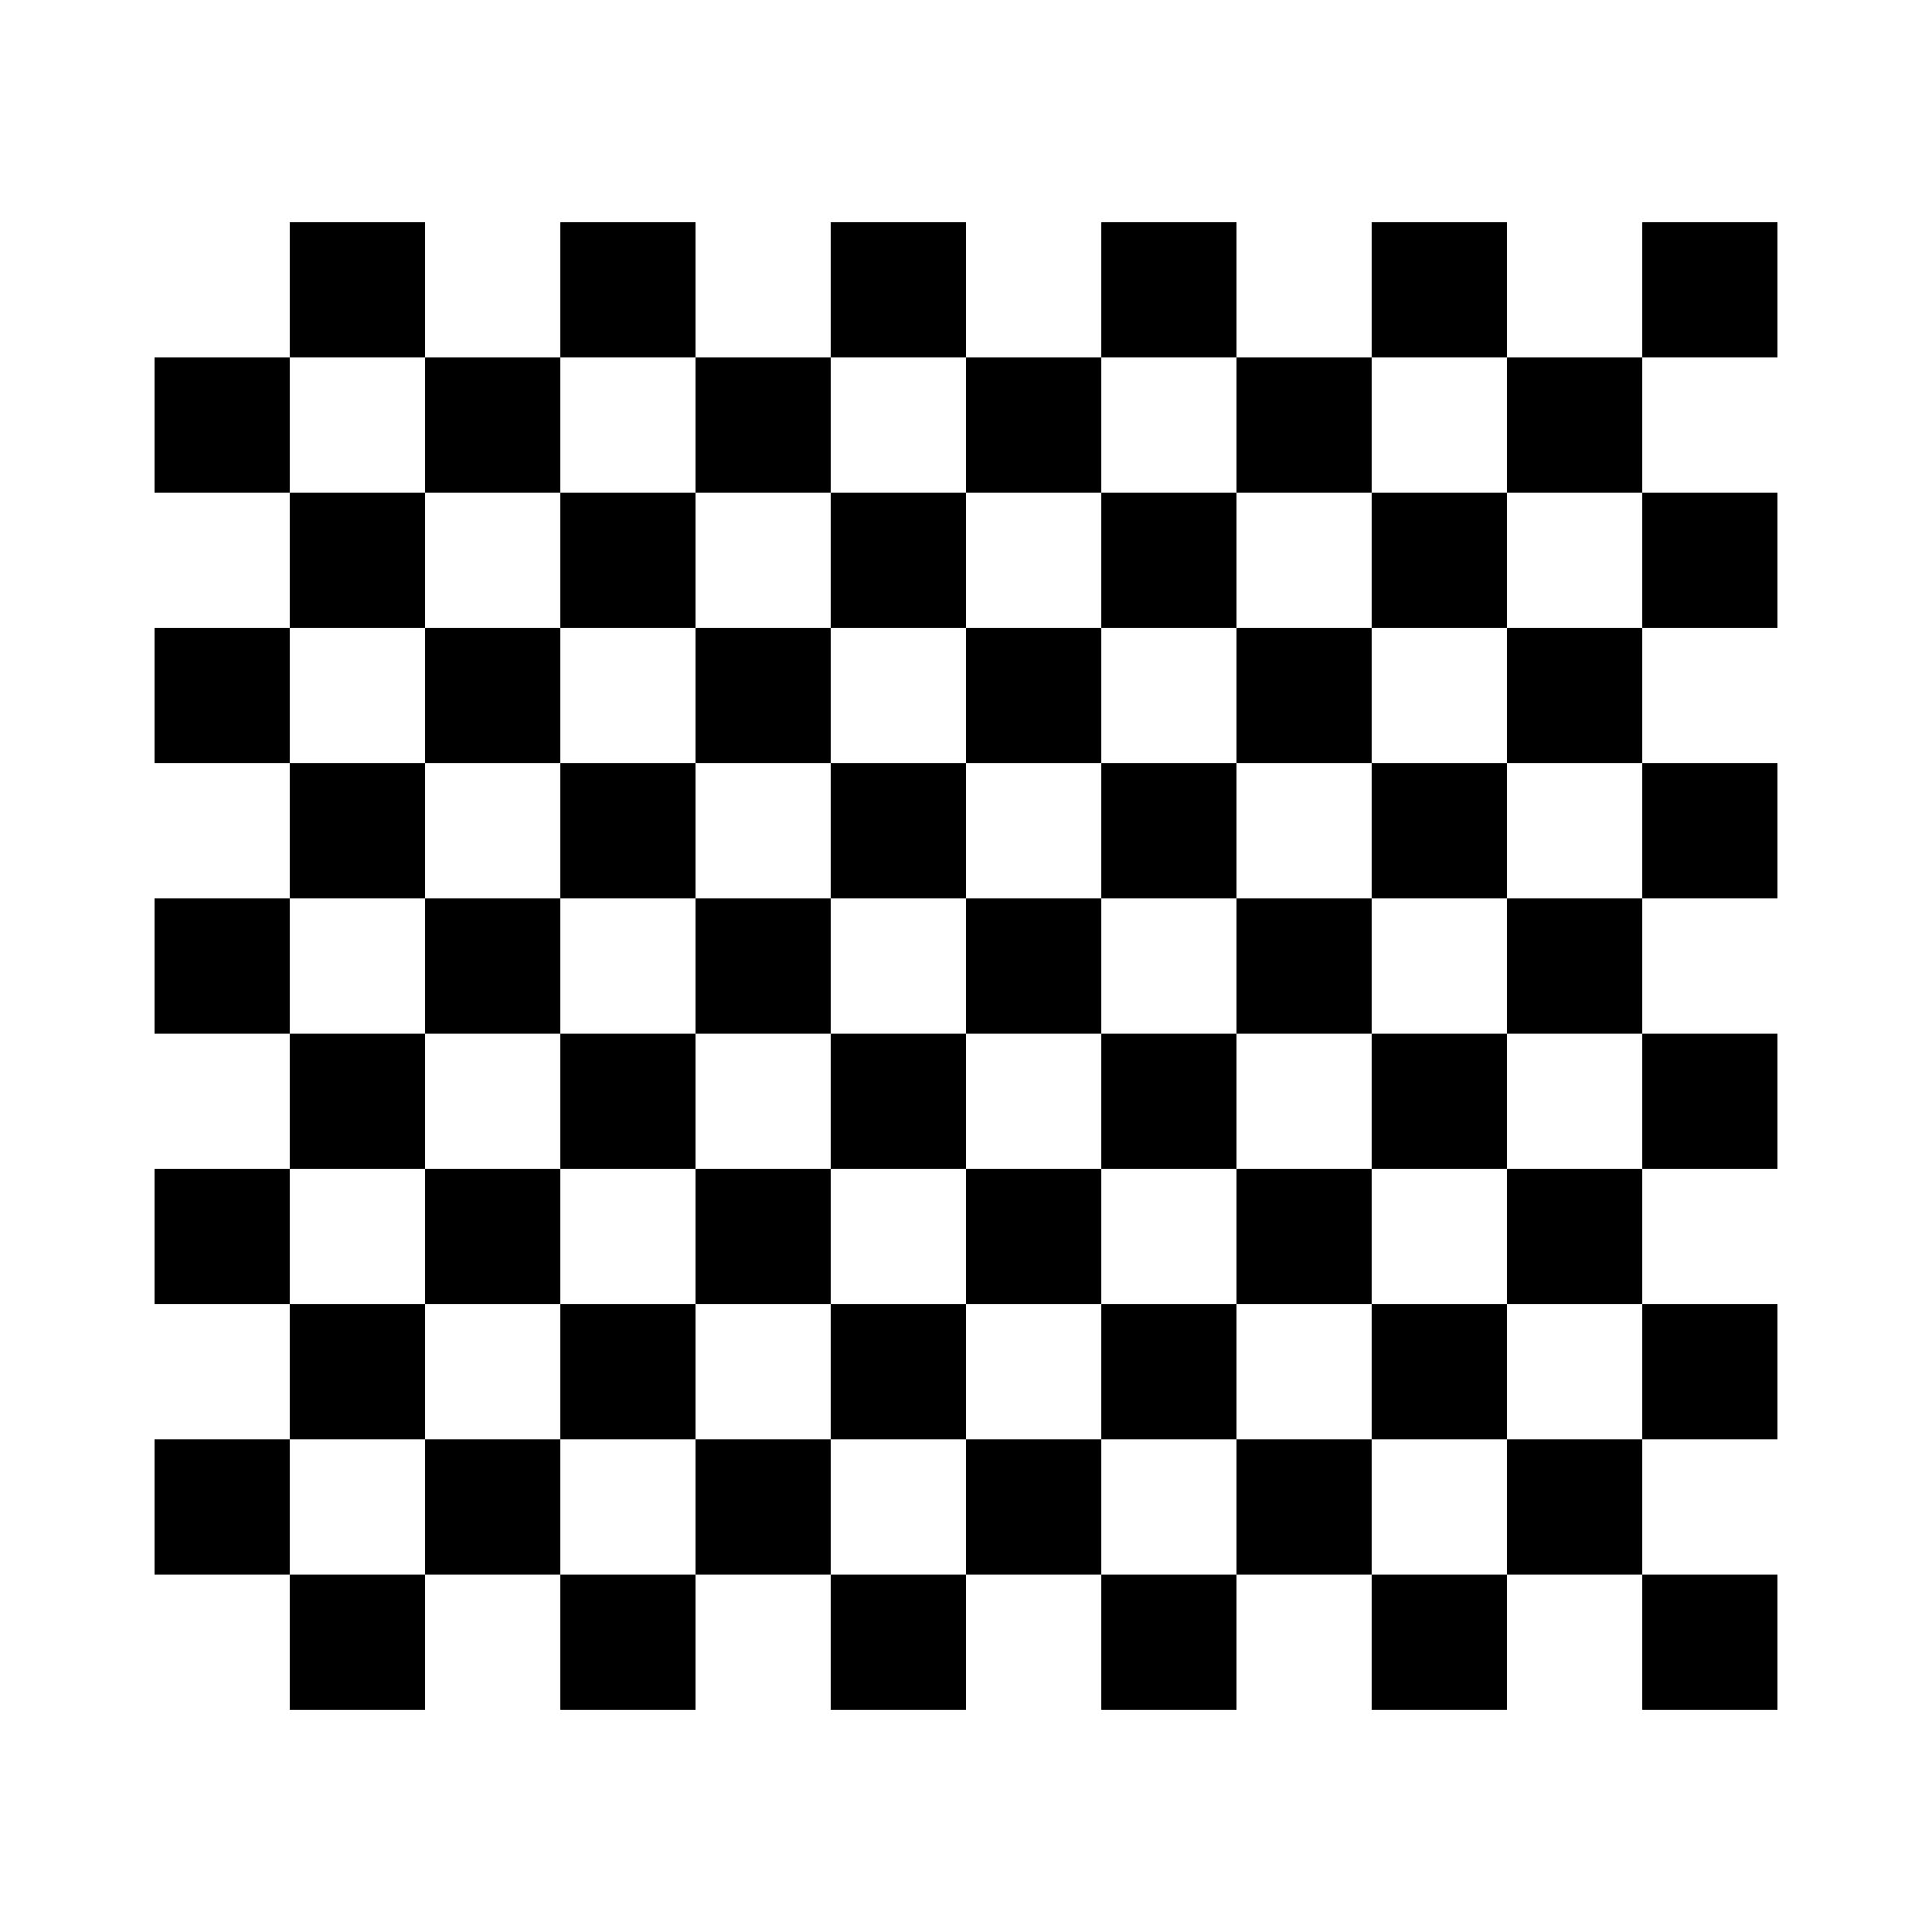
\includegraphics[scale=0.4]{checkerboard.png}
\caption{11 $\times$ 12 velika šahovnica.}
\end{figure}

Za učinkovito kalibracijo notranjih parametrov moramo zajeti okoli 10 - 20 slik z različnimi orientacijami in razdaljami šahovnice. Postopek kalibracije z orodjem je sledeč:
\begin{enumerate}
\itemsep0em
\item zajamemo slike šahovnice,
\item naložimo jih v orodje za kalibracijo,
\item izberemo število koeficientov za radialno popačenost (privzeto 2),
\item obkljukamo ali želimo oceniti poševnost in tangencialno popačenost,
\item kalibriramo,
\item postopek lahko ponavljamo s podmnožico slik na podlagi reprojekcijske napake,
\item ocenjene notranje parametre izvozimo za uporabo

\end{enumerate}
\begin{figure}[H]
\centering
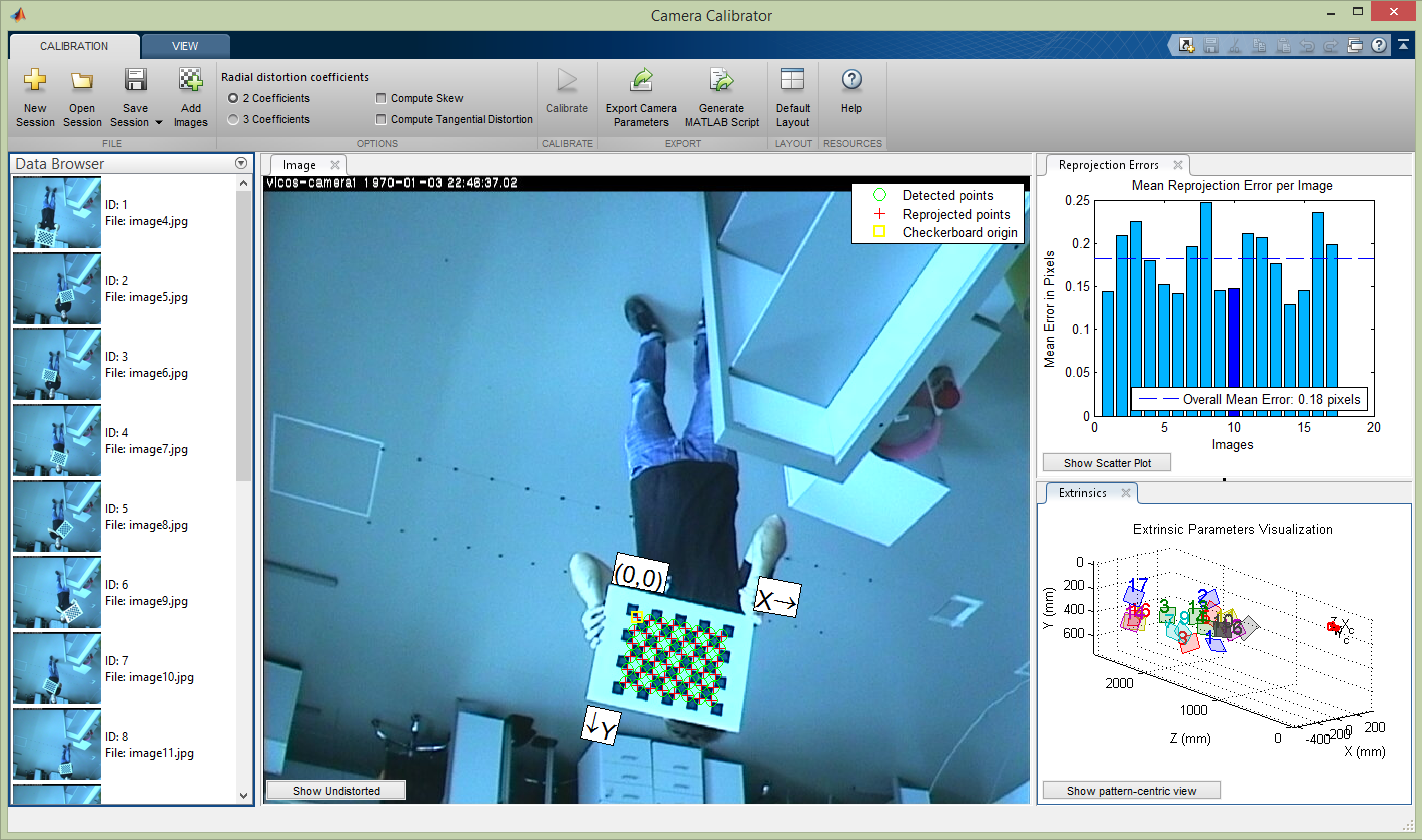
\includegraphics[width=\textwidth,height=\textheight,keepaspectratio]{internal_calibration.png}
\caption{Na sliki se vidi zaznane robove šahovnice in njena orientacija, graf reprojekcijske napake in vizualizacija zunanjih parametrov.}
\end{figure}

\begin{figure}[H]
\centering
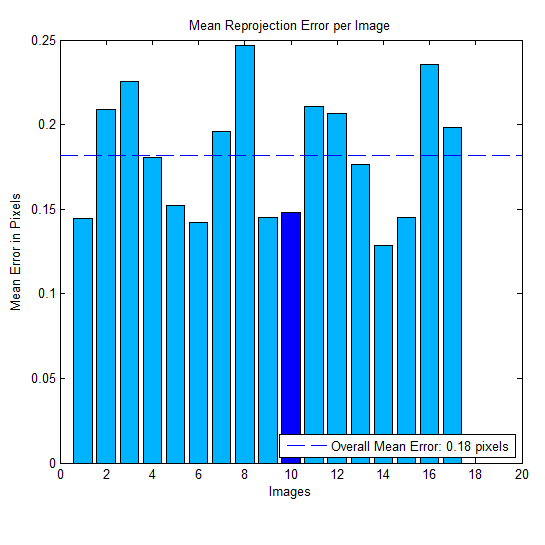
\includegraphics[scale=0.35]{reprojection_error.png}
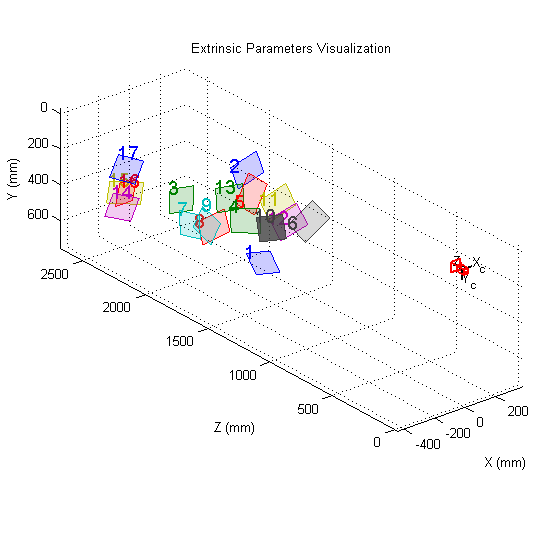
\includegraphics[scale=0.35]{extrinsic_visualization.png}
\caption{Graf reprojekcijske napake za vsako sliko (levo) in vizualizacija pozicij šahovnic s središčem v kameri (desno). }
\end{figure}

\begin{figure}[H]
\begin{align}
A &= 
\begin{bmatrix}
761,6027 & 0 & 386,6599 \\
0 & 835,939 & 362,0371 \\
0 & 0 & 1
\end{bmatrix} \\
\vec{r} &= [-0,2934 \ 0,1331] \\
\vec{t} &= [0.0006 \ 0,0012]
\end{align}
\caption{Primer ocenjenih notranjih parametrov ene izmed kamer. Tangencialna popačenost je skoraj zanemarljiva.}
\end{figure}


\subsection{Ocenjevanje zunanjih parametrov}
Ocenjevanje zunanjih parametrov je pravzaprav postavljanje kamere v nek skupen koordinatni sistem sveta. Določiti moramo torej rotacijsko matriko $R$ in translacijski vektor $\vec{T}$, ki predstavljata kje se nahaja koordinatni sistem glede na kamero. Za oceno parametrov uporabimo metodo, ki je opisana v poglavju \ref{externalparamssection}. Potrebujemo le eno sliko na kateri lahko določimo točke v svetu. Za potrebe diplomskega dela sem v sobi na tleh označil in določil svoj koordinatni sistem. Med oznakami po $x$ osi je razdala $20 \ cm$, na $y$ osi pa $60 \ cm$. Enota je $1 \ cm$.

\begin{figure}[H]
\centering
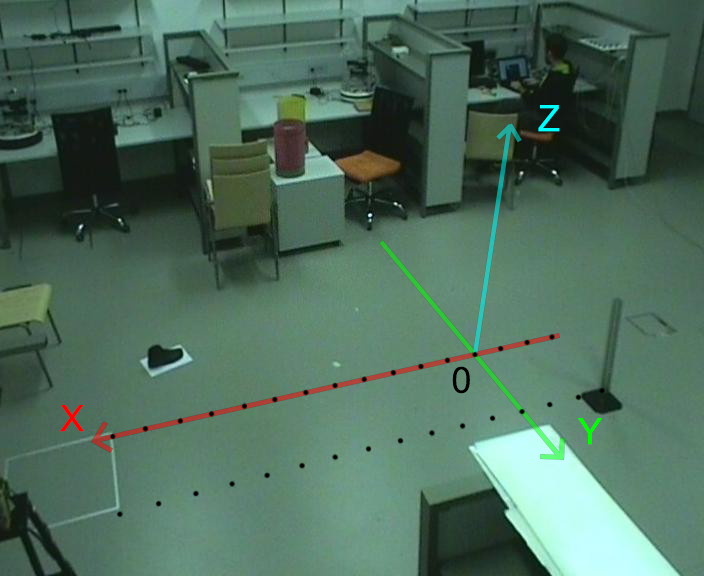
\includegraphics[width=\textwidth,height=\textheight,keepaspectratio]{coord_system.png}
\caption{Na sliki se vidi označen koordinatni sistem sveta. Točke označene s črnimi pikami so koplanarne in z njimi določimo zunanje parametre kamere.}
\label{coordsystemimg}
\end{figure}

Najprej moramo določiti pare $(\vec{X}, \vec{X'})$, ki določajo preslikavo med točko v svetu in točko na sliki. Imeti moramo minimalno 6 parov, ker moramo oceniti 12 parametrov (9 za rotacijsko matriko in 3 za translacijo), en par pa nam določi 2 linearno neodvisni enačbi. Točke v svetu določimo sami, nato pa jih ročno ali avtomatsko označimo na sliki. Sam sem določil 16 parov, s katerimi sem ocenil zunanje parametre. Če je slika kakorkoli popačena, jo moramo popraviti.

\begin{table}[H]
\centering
\begin{tabular}{| c | c | c | c | c |}
\hline
x & y & z & x' & y' \\
\hline
240 & 0 & 0 & 591.1441 & 139.8898 \\
200 & 0 & 0 & 523.8898 & 156.1610 \\
160 & 0 & 0 & 460.9746 & 171.3475 \\
120 & 0 & 0 & 399.1441 & 185.4492 \\
80 & 0 & 0 & 340.5678 & 198.4661 \\
40 & 0 & 0 & 284.1610 & 211.4831 \\
0 & 0 & 0 & 229.9237 & 223.4153 \\
-40 & 0 & 0 & 177.8559 & 234.2627 \\
240 & 60 & 0 & 584.6356 & 62.8729 \\
200 & 60 & 0 & 508.7034 & 83.4831 \\
160 & 60 & 0 & 437.1102 & 101.9237 \\
120 & 60 & 0 & 368.7712 & 119.2797 \\
80 & 60 & 0 & 303.6864 & 135.5508 \\
40 & 60 & 0 & 241.8559 & 150.7373 \\
0 & 60 & 0 & 183.2797 & 165.9237 \\
-40 & 60 & 0 & 125.7881 & 177.8559 \\
\hline
\end{tabular}
\caption{16 parov točk dobljenih iz slike \ref{coordsystemimg}.}
\label{pointpairs}
\end{table}

Iz zgornje tabele se lepo vidi, da so vse točke v svetu koplanarne, saj je pri vseh $z = 0$. Sedaj lahko določimo matriko $B$, ki je za eno par točk definirana v enačbi \eqref{bmatrix}. Za vsak par točk dodamo nove vrstice matriki $B$ in tako dobimo matriko velikosti $2n \times 12$ oz. $3n \times 12$ (če izračunamo tudi zadnjo vrstico, ki je redundantna), kjer je $n$ število parov točk. Zavedati se moramo, da so $u, v, w$ določeni z enačbo \eqref{uvw}, kjer uporabimo matriko notranjih parametrov $A$. S tem korakom odstranimo matriko $A$ iz matrike $A * [R|\vec{T}]$ in s tem lažje določimo matriko $[R|\vec{T}]$. Z razcepom na singularne vrednosti (SVD) rešimo sistem $B * \vec{p} = 0$ in dobljeno rešitev preoblikujemo v $3 \times 4$ matriko zunanjih parametrov. Rešitev je pravzaprav deveti stolpec matrike $V$, ki jo vrne SVD razcep in ne dvanajsti kot je opisano pri izpeljavi teorije. To je posledica koplanarnosti svetovnih točk. Matrika $B$ je ranga 9, ker je $z$ komponenta vseh točk v svetu enaka 0. Spodnja matrika prikazuje primer rešitve za pare točk iz tabele \ref{pointpairs}.
\begin{equation}
[R|\vec{T}] = 
\begin{bmatrix}
-0.0018 & 0.0006 & 0 & 0.1989 \\
0.0003 & 0.0007 & 0 & 0.1607 \\
0.0005 & 0.0016  & 0 & -0.9668 \\
\end{bmatrix}
\end{equation}

Hitro opazimo, da podmatrika $R$ ni prav nič podobna rotacijski matriki. Stolpci rotacijskih matrik so paroma ortonormirani. Ker računamo s homogenimi koordinatami, lahko dobljeno matriko pomnožimo z neničelnim skalarjem brez, da bi pri tem uničili model kamere. Sedaj lahko ročno popravimo podmatriko $R$, da bo karseda podobna rotacijski matriki.
\begin{align}
[R|\vec{T}] = [\vec{R_1} \ \vec{R_2} \ \vec{R_3} \ \vec{T}] &\sim \frac{1}{||R_1||} * 
\begin{bmatrix}
-0.0018 & 0.0006 & 0 & 0.1989 \\
0.0003 & 0.0007 & 0 & 0.1607 \\
0.0005 & 0.0016  & 0 & -0.9668 \\
\end{bmatrix} \\
[R|\vec{T}] &\sim
\begin{bmatrix}
-0.9544 & 0.3003 & 0 & 106.6226 \\
0.1419 & 0.3877 & 0 & 86.1440 \\
0.2627 & 0.8810 & 0 & -518.2979 \\
\end{bmatrix}
\end{align}

Sedaj sta prva dva stolpca ortonormirana oz. skoraj ortonormirana (odvisno od natančnosti ocene parametrov). Sedaj je čas, da naslovimo še zadnji problem rotacijske matrike. Zaradi prej omenjene koplanarnosti je tretji stolpec ničelni vektor. Vemo, da mora biti paroma ortonormiran s prvima stolpcema, zato ga lahko določimo z vektorskim produktom.

\begin{align}
R_3 &= R_1 \times R_2 =
\begin{bmatrix}
-0.9544 \\
0.1419 \\
0.2627
\end{bmatrix}
\times
\begin{bmatrix}
0.3003 \\
0.3877 \\
0.8810
\end{bmatrix} \\
R_3 &= 
\begin{bmatrix}
0.0232 \\
0.9197 \\
-0.4127
\end{bmatrix}
\end{align}

Sedaj moramo le še določiti pravo smer novo izračunanega vektorja. $R_3$ kot tudi $-R_3$ sta legalni rešitvi in implicitno določata sučnost koordinatnega sistema. Sam sem pravilno rešitev določil ročno na podlagi projekcije točk, kot je vidno iz slike \ref{reprojectionwrongimg}.

\begin{figure}[H]
\centering
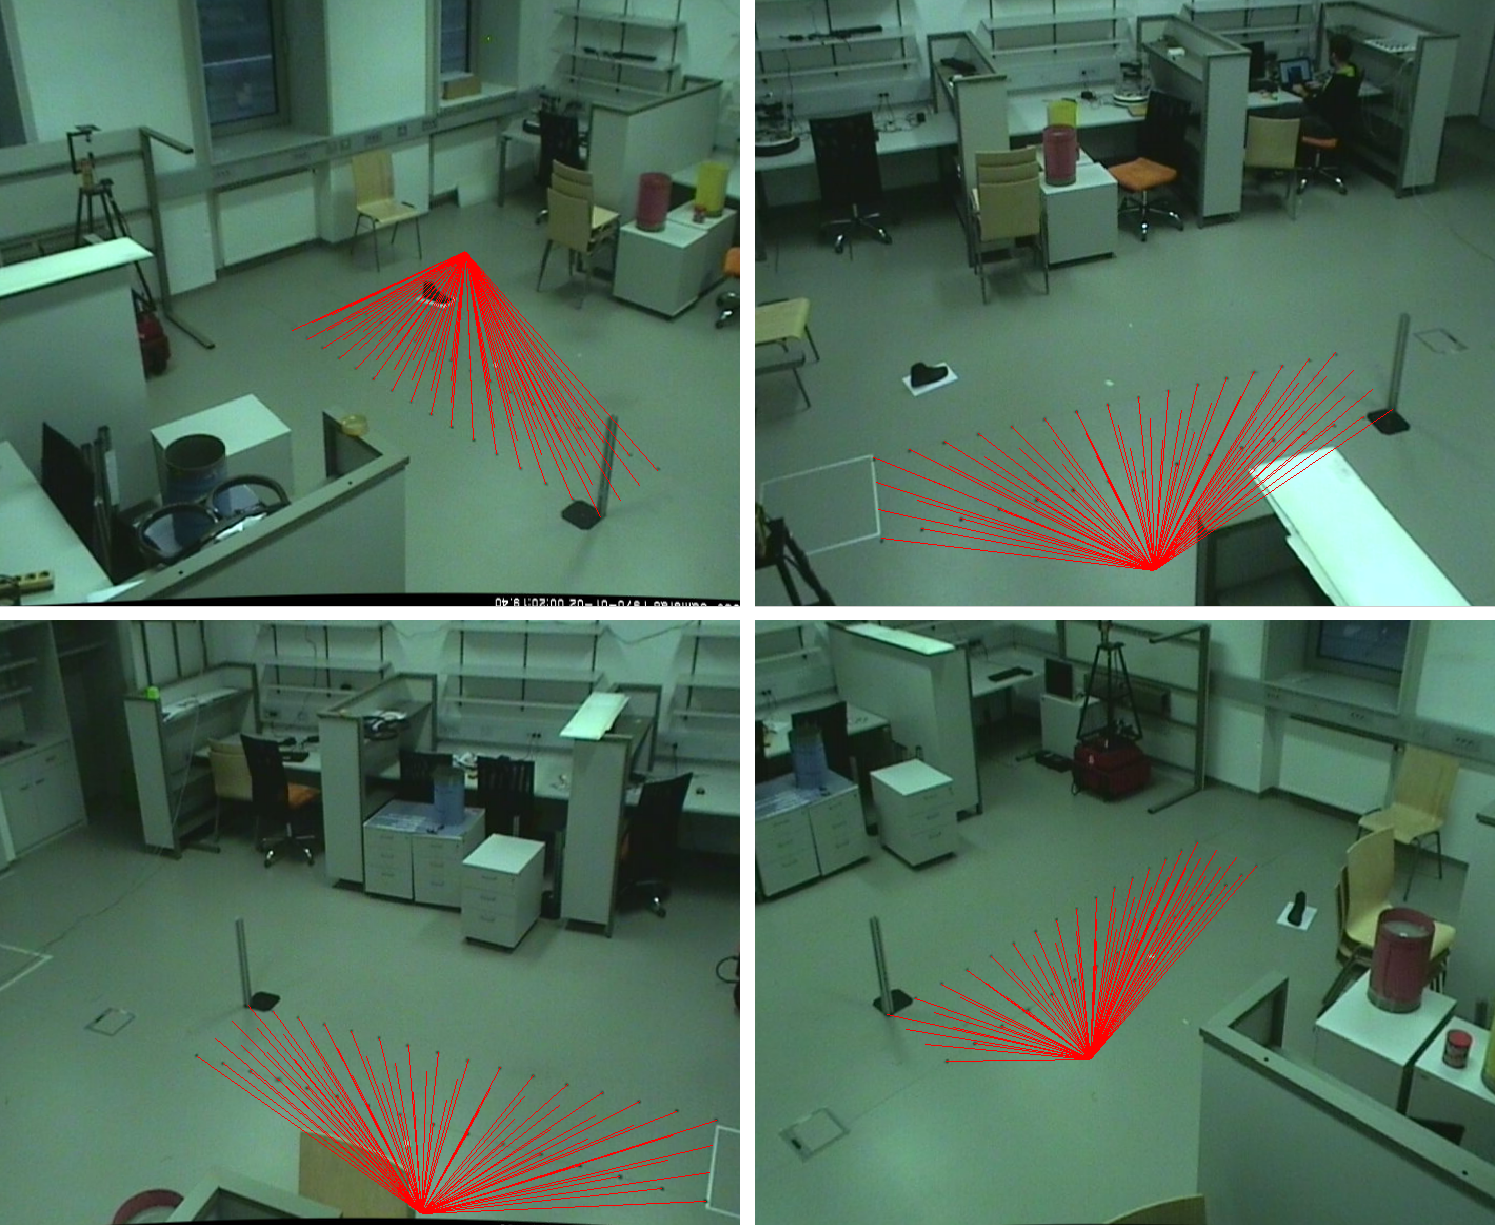
\includegraphics[scale=0.25]{reprojection_wrong.png}
\caption{Projekcija piramide na sliko pokaže, da so prvi trije koordinatni sistemi levosučni, zato moramo obrniti smer zadnjega stolpca matrike $R$.}
\label{reprojectionwrongimg}
\end{figure}

\begin{figure}[H]
\centering
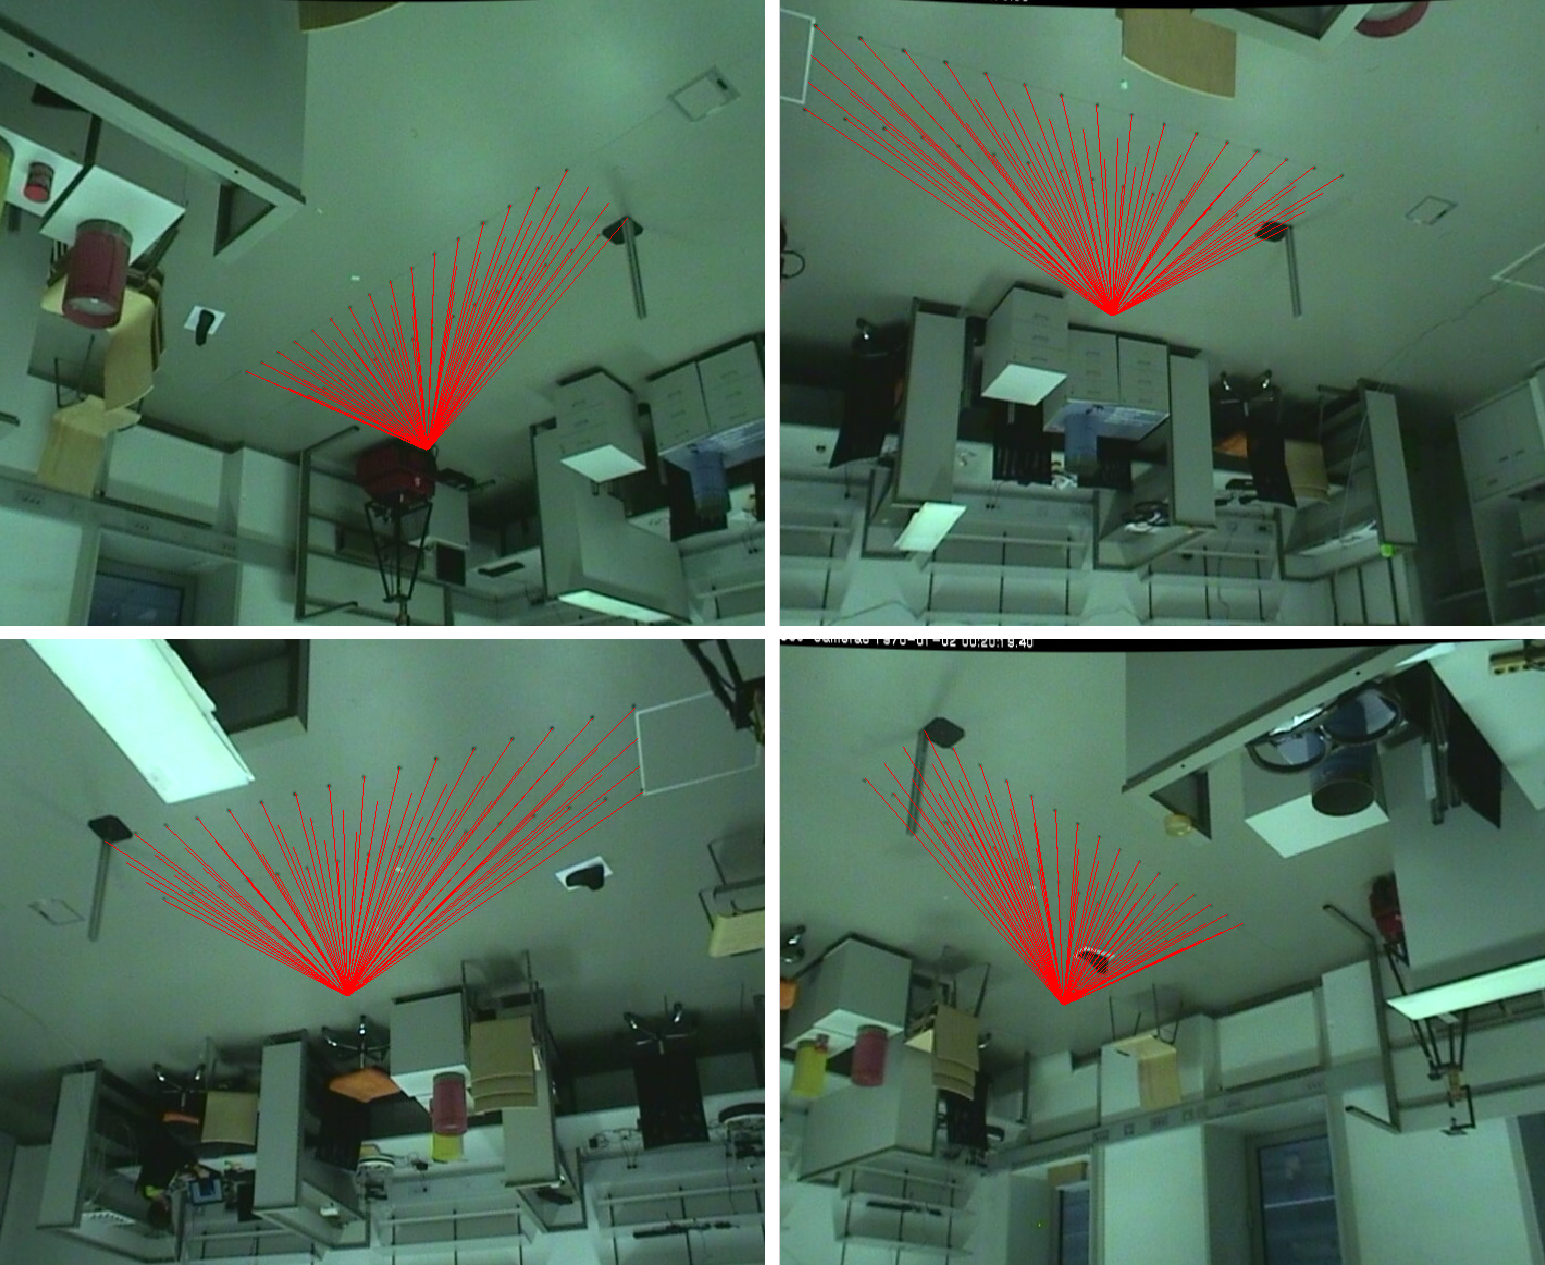
\includegraphics[scale=0.25]{reprojection_corrected.png}
\caption{Na novo ocenjeni zunanji parametri pravilno modelirajo kamere, kar je razvidno iz projekcije piramide.}
\end{figure}

Končna matrika zunanjih parametrov za točke iz tabele \ref{pointpairs} je,
\begin{equation}
[R|\vec{T}] = 
\begin{bmatrix}
-0.9544 & 0.3003 & 0.0232 & 106.6226 \\
0.1419 & 0.3877 & 0.9197 & 86.1440 \\
0.2627 & 0.8810 & -0.4127 & -518.2979 
\end{bmatrix}
\end{equation}

Stolpci rotacijske matrike so le približno paroma ortonormirani, kar je posledica vnašanja napak pri ročnem določanju koordinatnega sistema. Če bi matriko prisilno ortonormirali bi prišlo do večje reprojekcijske napake. 

\section{Implementacija zaznavanja označevalnika}
Za zaznavanje označevalnika uporabljam postopek opisan v poglavju \ref{markersection}. Za prag sem določil RGB interval, ker je označevalnik izrazito rumene barve. Spodnja meja intervala je $[220 \ 220 \ 0]$, zgornja pa $[255, 255, 200]$. V prosotoru ne sme prihajati do velikih sprememb v osvetljenosti, zato imajo kamere nastavljen fiksni kontrast, dnevna svetloba pa je izolirana od prostora. Spodaj so prikazane slike posameznih faz zaznavanja.

\begin{figure}[H]
\centering
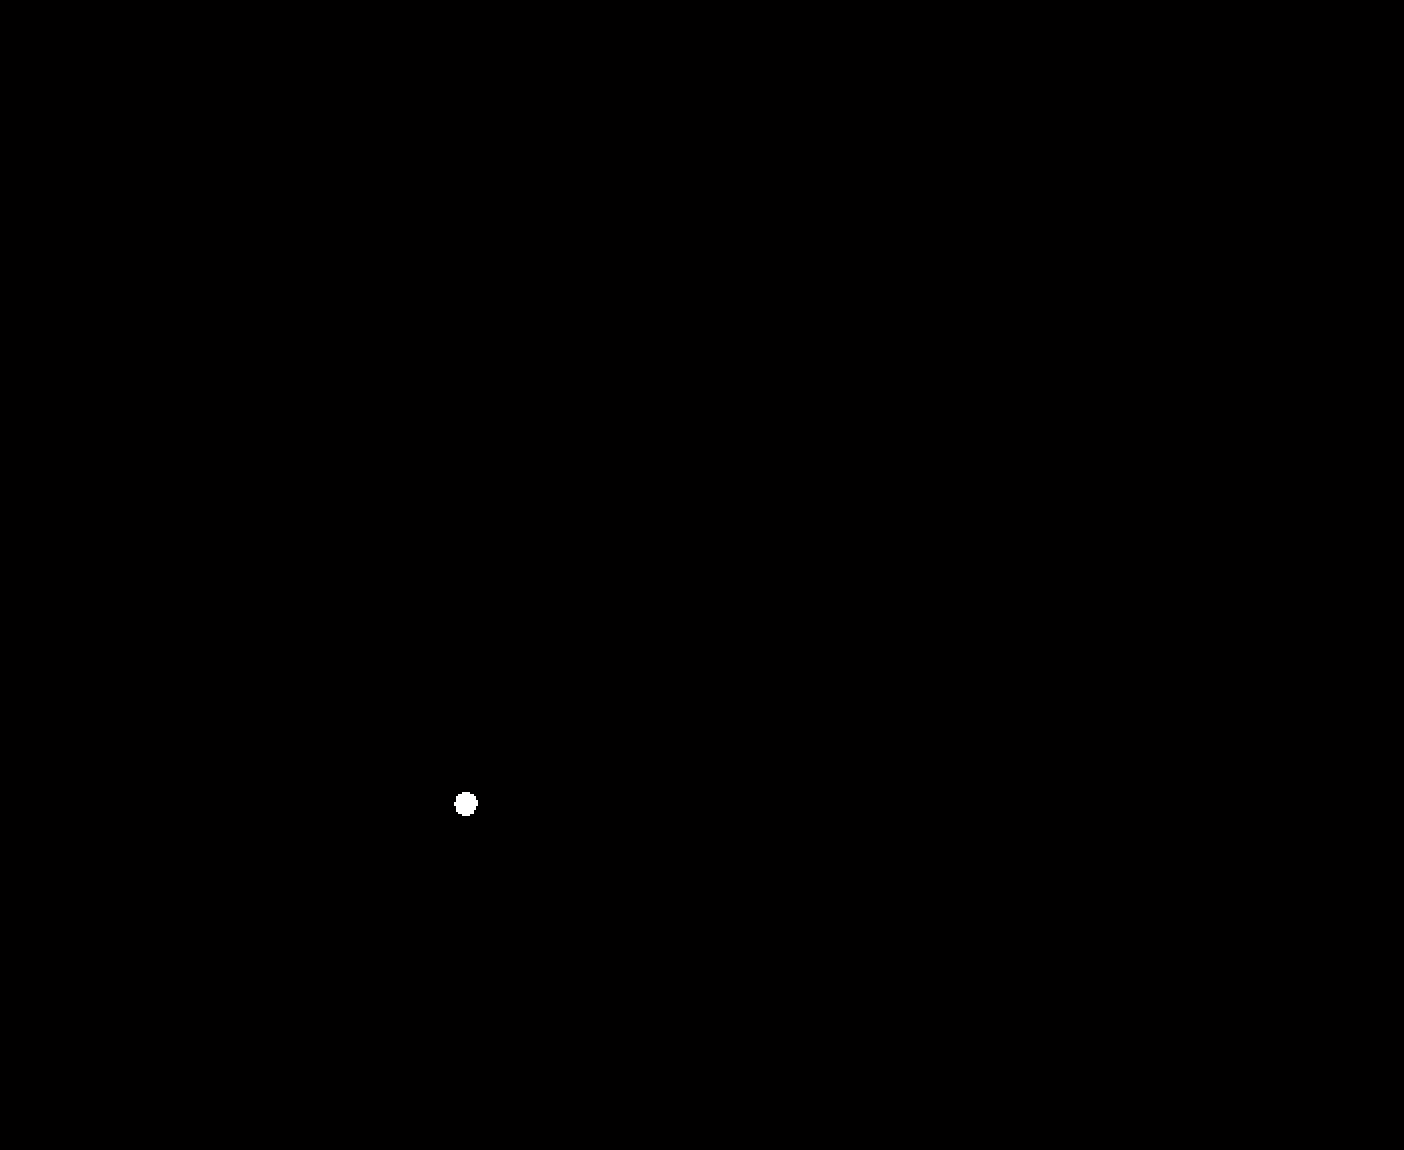
\includegraphics[width=\textwidth,height=\textheight,keepaspectratio]{segmented.png}
\caption{Segmentacija zajete slike z belo barvo označuje zaznan označevalnik.}
\end{figure}

\begin{figure}[H]
\centering
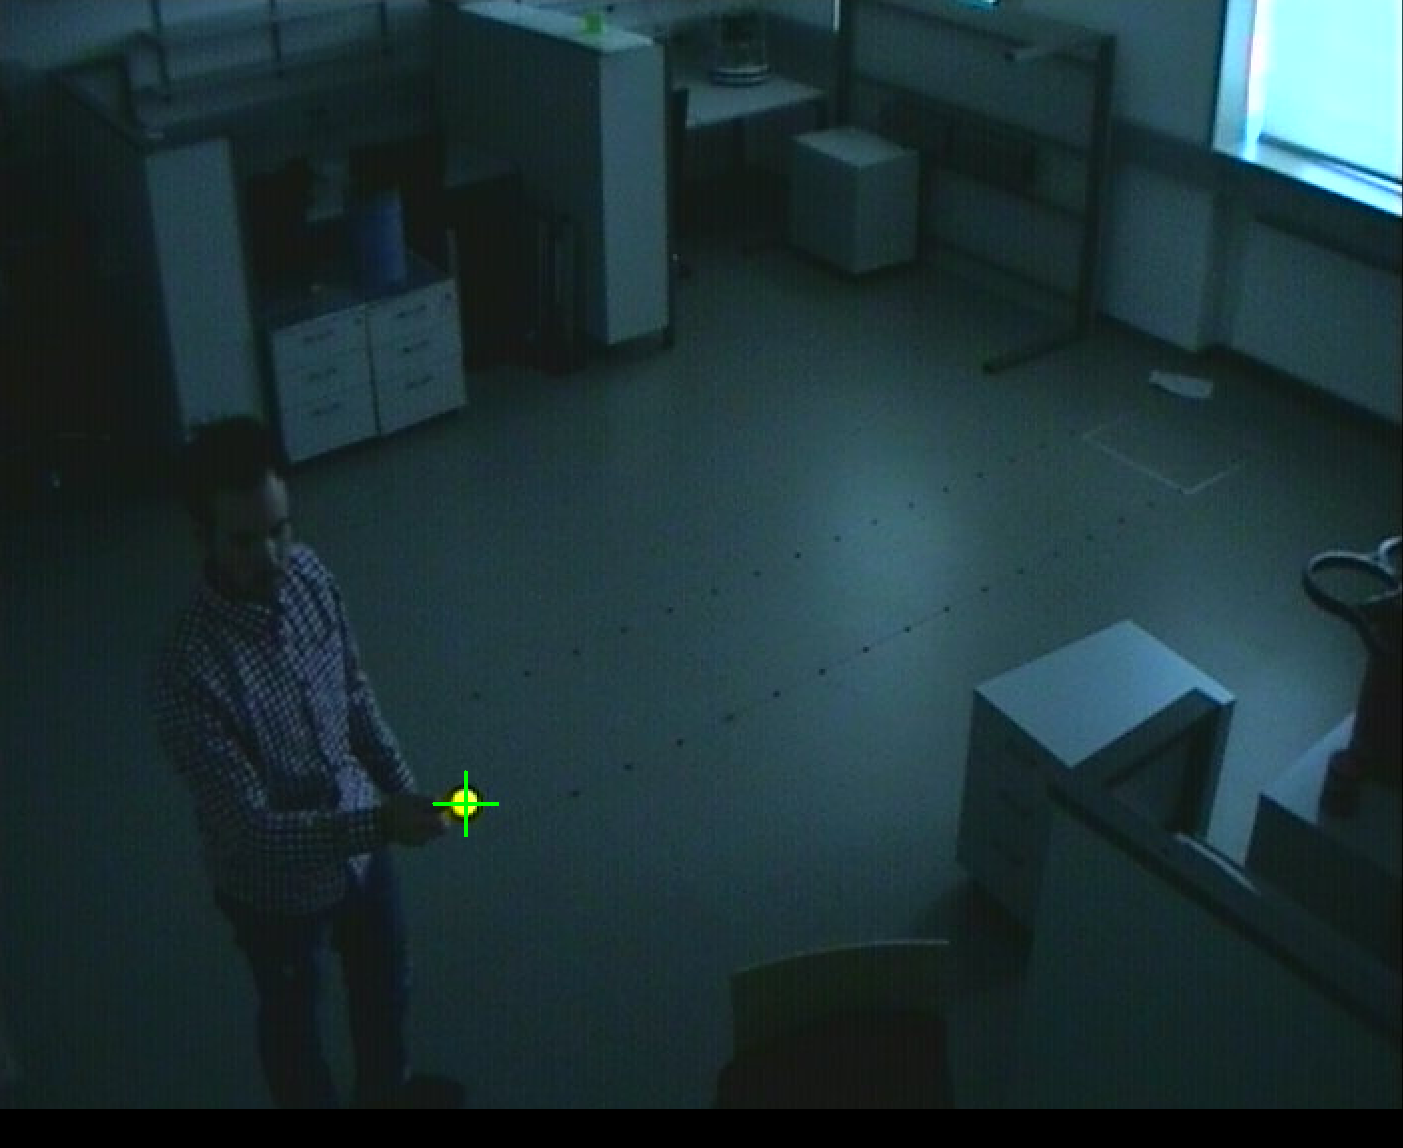
\includegraphics[width=\textwidth,height=\textheight,keepaspectratio]{detected.png}
\caption{Pozicijo označevalnika na sliki (zeleni +) dobimo z masnim središčem segmenta.}
\end{figure}

\section{Postavitev sistema}
V prostoru z dimenzijami $7,4 \times 7,7 \times 2,97 \ m^3$ so bile na strop pritrjene štiri Axis 215 PTZ kamere. Sistem deluje v realnem času s 24 meritvami na sekundo. Spodnja slika ilustrira postavitev in orientacijo kamer ter njihovo oštevilčenost.

\begin{figure}[H]
\centering
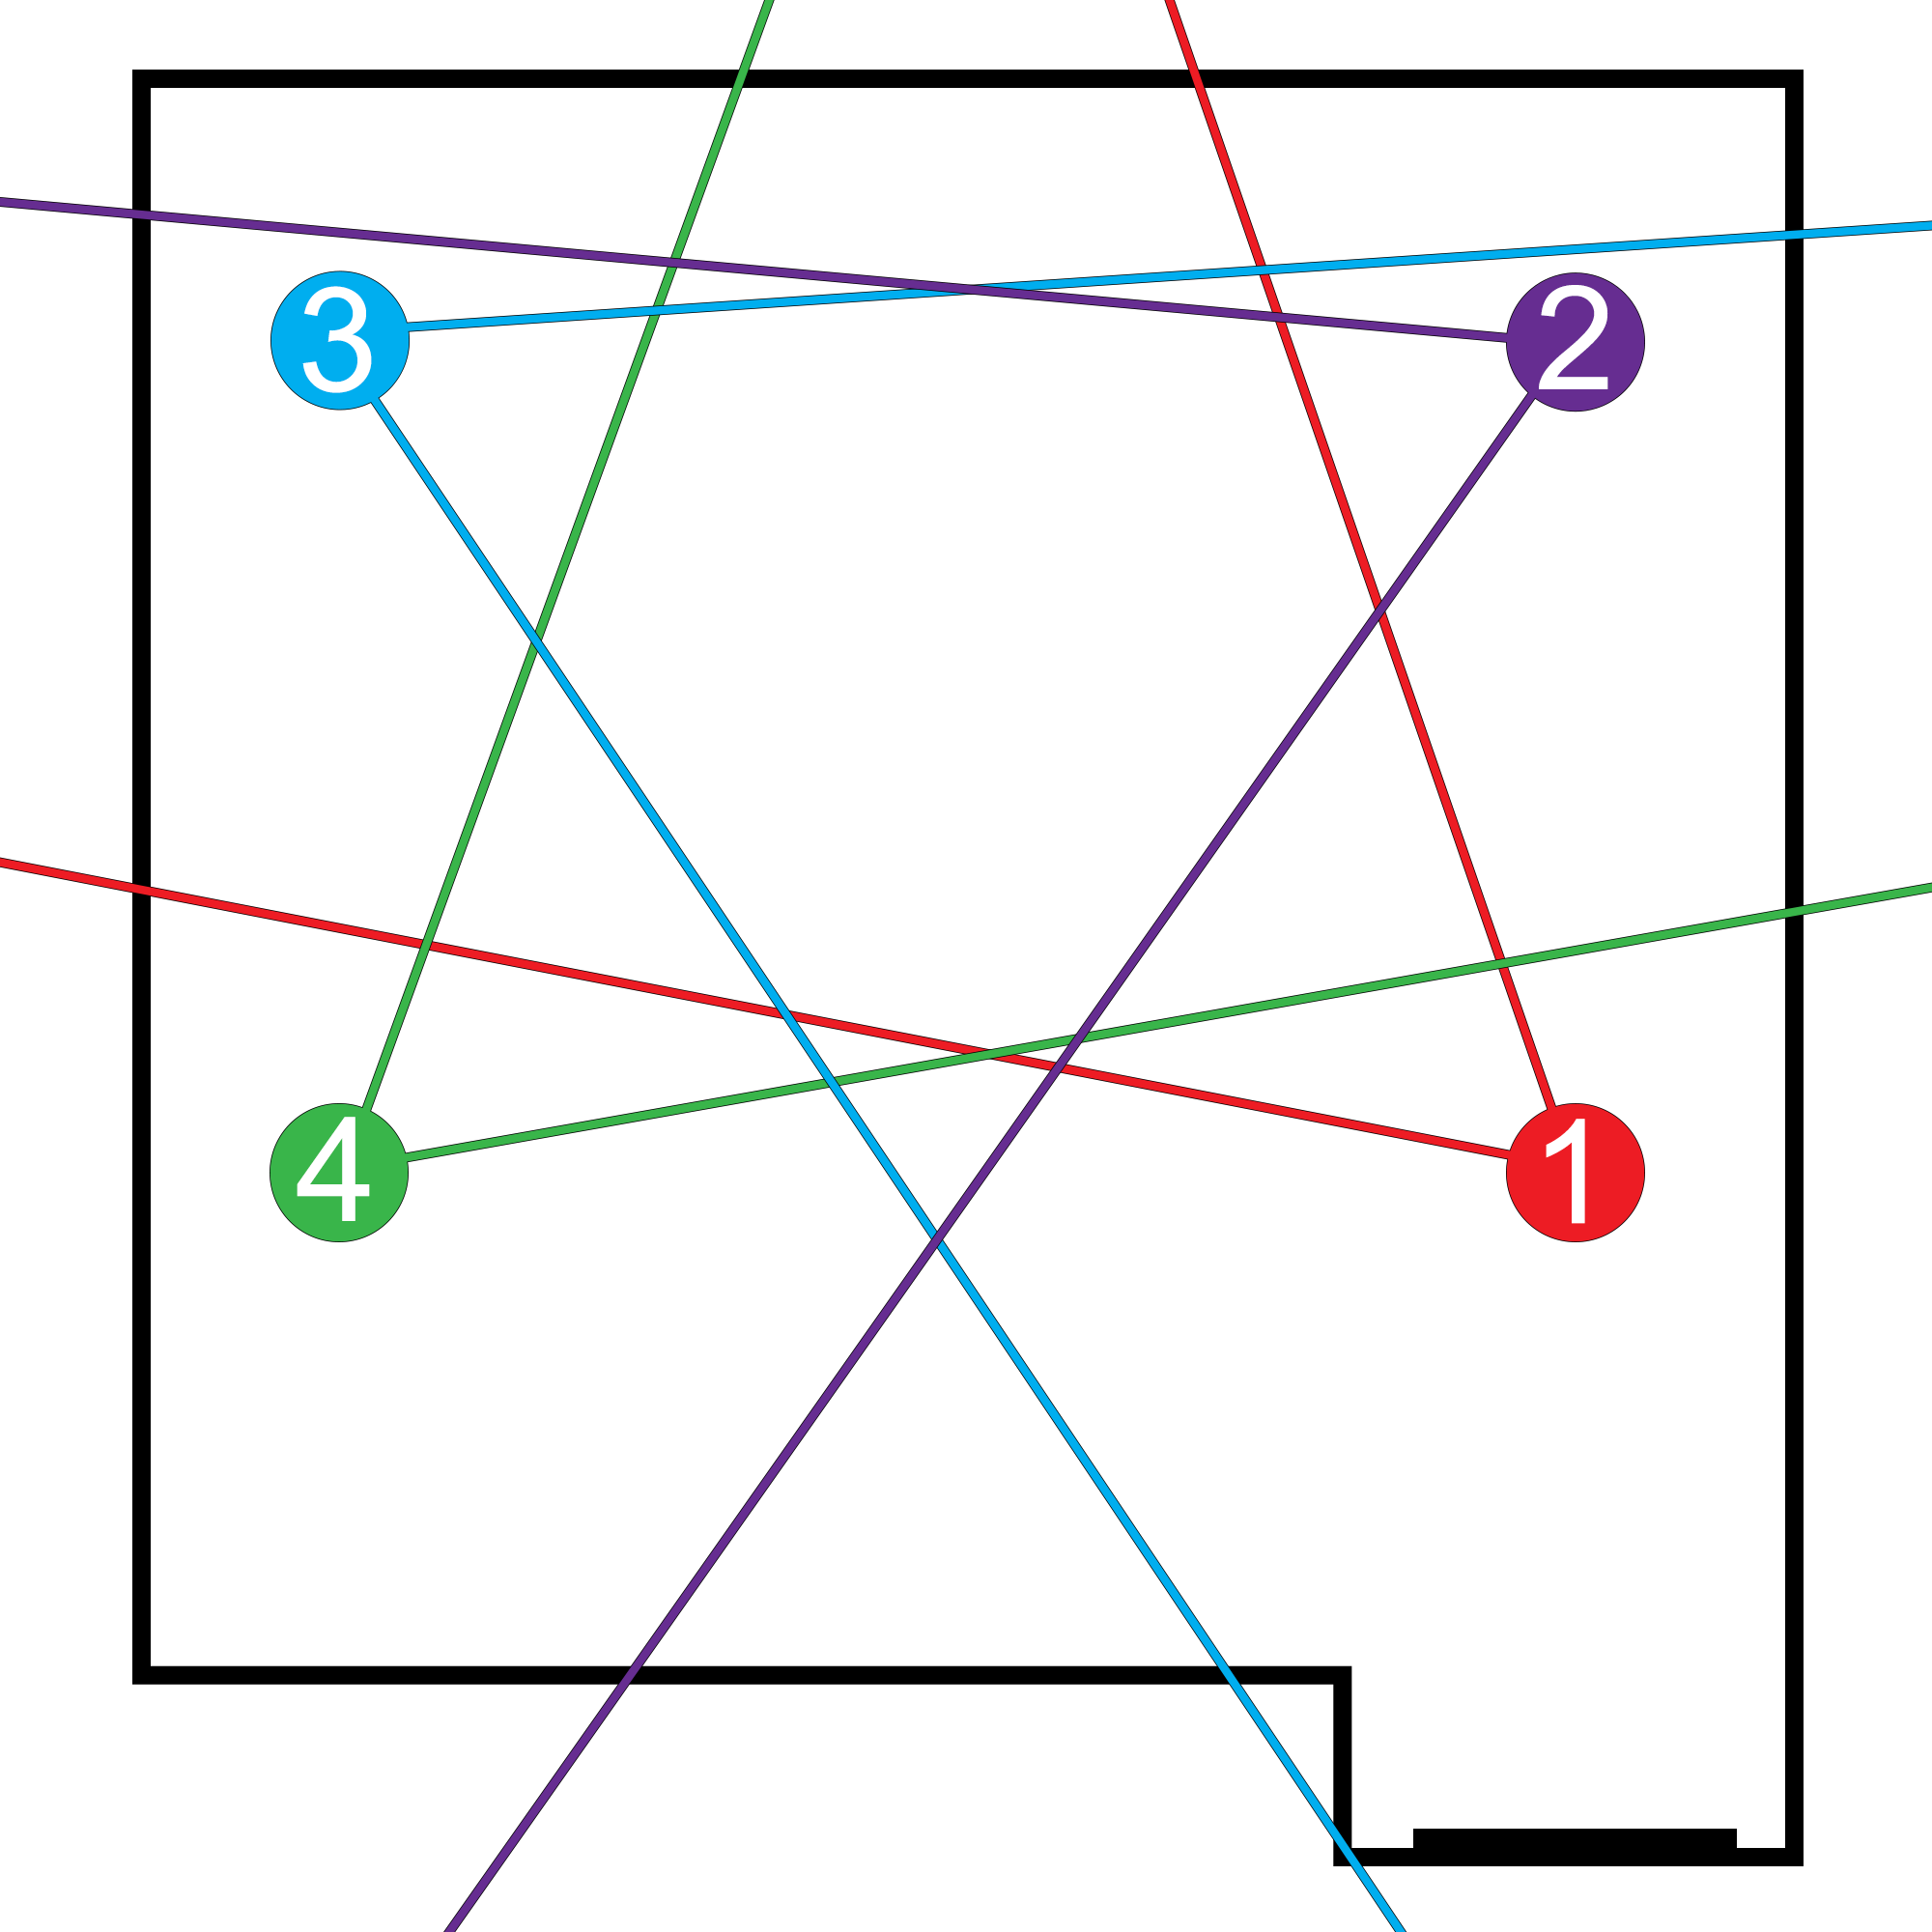
\includegraphics[scale=0.5]{room_setting.png}
\caption{Kamere v prostoru.}
\end{figure}

Kamere so preko ethernet omrežje povezane v zvezdišče in nato v brezžični usmerjevalnik. Prenosni računalnik je v omrežje povezan brezžično. Na računalniku teče glavni program, ki komunicira s kamerami in računa položaj označevalnika v prostoru. Topologijo povezave predstavlja spodnja slika.
\begin{figure}[H]
\centering
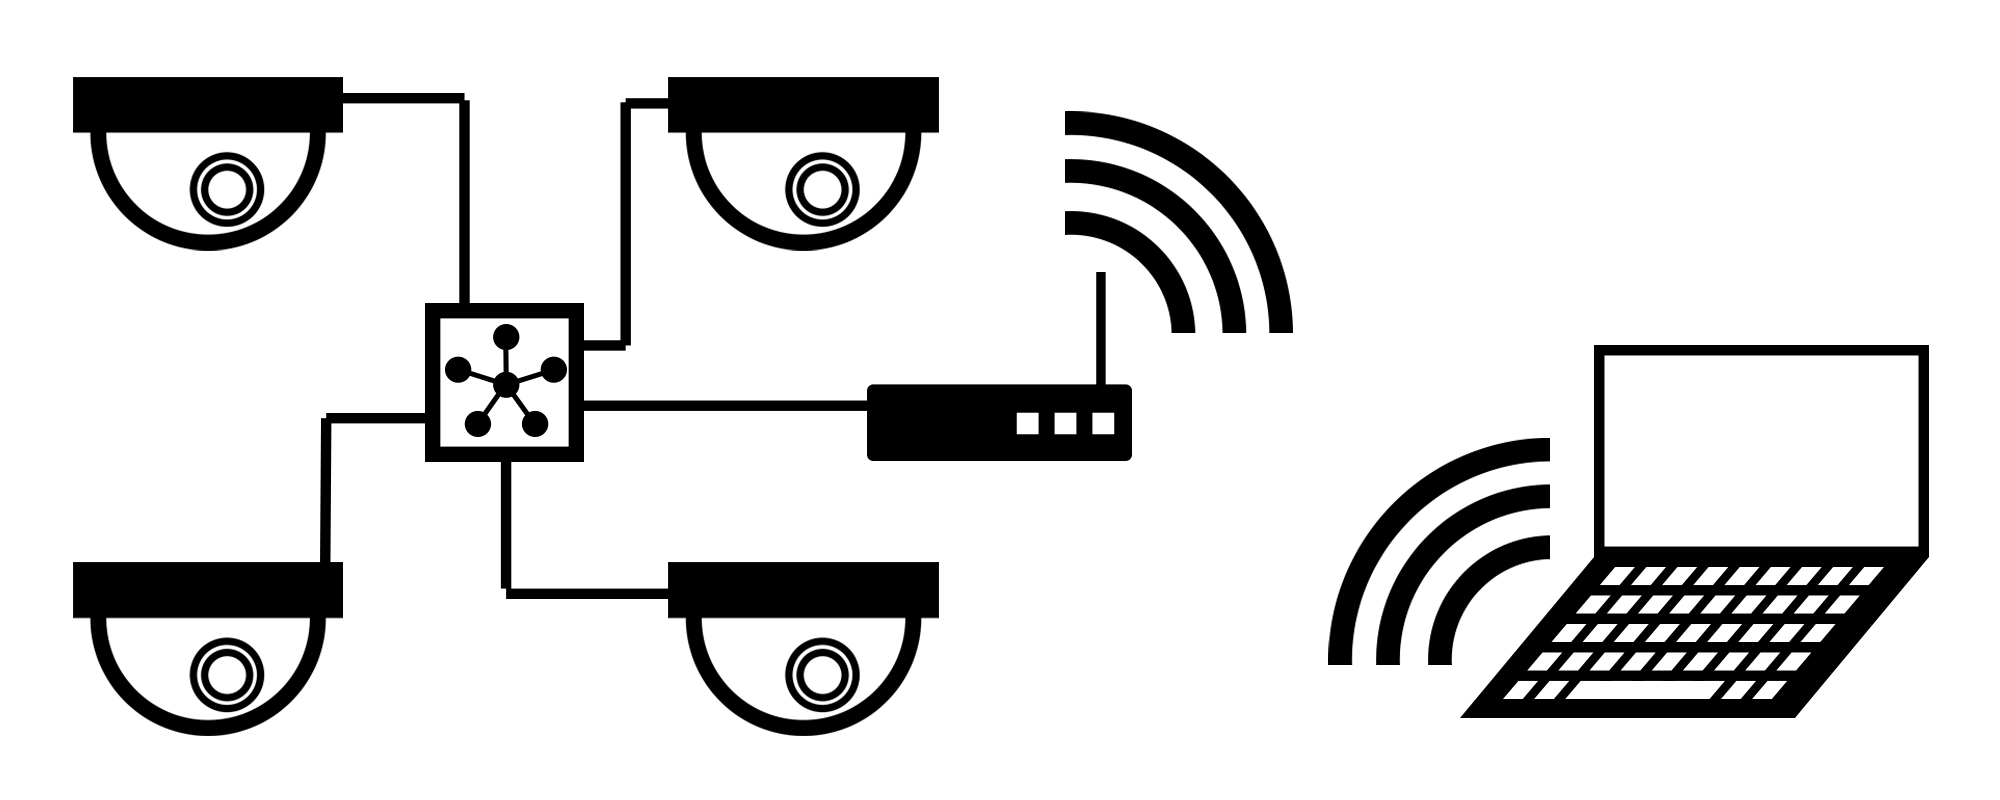
\includegraphics[width=\textwidth,height=\textheight,keepaspectratio]{topology.png}
\caption{Topologija povezave.}
\end{figure}

Proces zaznavanja položaja je razdeljen v preproste korake, ki jih opisuje spodnja psevdo koda.

\begin{lstlisting}
Glavni proces: 
  Zazeni n podprocesov, kjer je n stevilo kamer.
  Ponavljaj:
    Za vsak podproces:
      Sprejmi tocko oznacevalnika.
      Dopolni matriko za triangulacijo.
    Ce vsaj dve kameri zaznata oznacevalnik:
      Trianguliraj polozaj oznacevalnika v prostoru.
      Izpisi polozaj.

Podproces:
  Vzpostavi komunikacijo s kamero.
  Inicializiraj privzete parametre kamere.
  Ponavljaj:
    Zajemi sliko iz kamere.
    Zaznaj oznacevalnik.
    Sporoci tocko oznacevalnika glavnemu procesu.
\end{lstlisting}

\chapter{Rezultati}
\section{Reprojekcija kalibracijskih točk}

Povprečna reprojekcijska napaka pri kalibriranju notranjih parametrov je med 0.14 in 0.16 slikovnih pik. To je posledica selektivne izbire slik s katerimi zavestno zmanjšamo napako. Napaka pod 1 slikovnim elementom, je pri delu s slikami zelo dobra. Bolj zanimiva je reprojekcija kalibracijskih točk zunanjih parametrov. Točke na slikah so bile določene ročno z ločljivostjo meritve 1 slikovnega elementa. Pomemben faktor pri tem postopku je vnos človeške napake. Sistem se je kljub napakam kalibriral tako, da je vsota razlik kvadratov najmanjša. 

\begin{table}[H]
\centering
\begin{tabular}{| l | c | c |}
\hline
 & povprečna napaka & varianca povprečne napake \\
\hline
kamera 1 & 0.8542 & 0.2965 \\
kamera 2 & 0.8739 & 0.1146 \\
kamera 3 & 0.9786 & 0.6938 \\
kamera 4 & 0.8289 & 0.1011 \\
\hline
\end{tabular}
\caption{Povprečna napaka reprojekcije kalibracijskih točk zunanjih parametrov. Napake so merjene v slikovnih elementih.}
\label{pointpairs}
\end{table}

Opazimo lahko, da so povprečne napake dokaj konsistentne pri okoli 0.9 slikovnega elementa. Pri tretji kameri izstopa varianca, kar je lahko posledica slabšega ročnega določanja točk.

\begin{figure}[H]
\centering
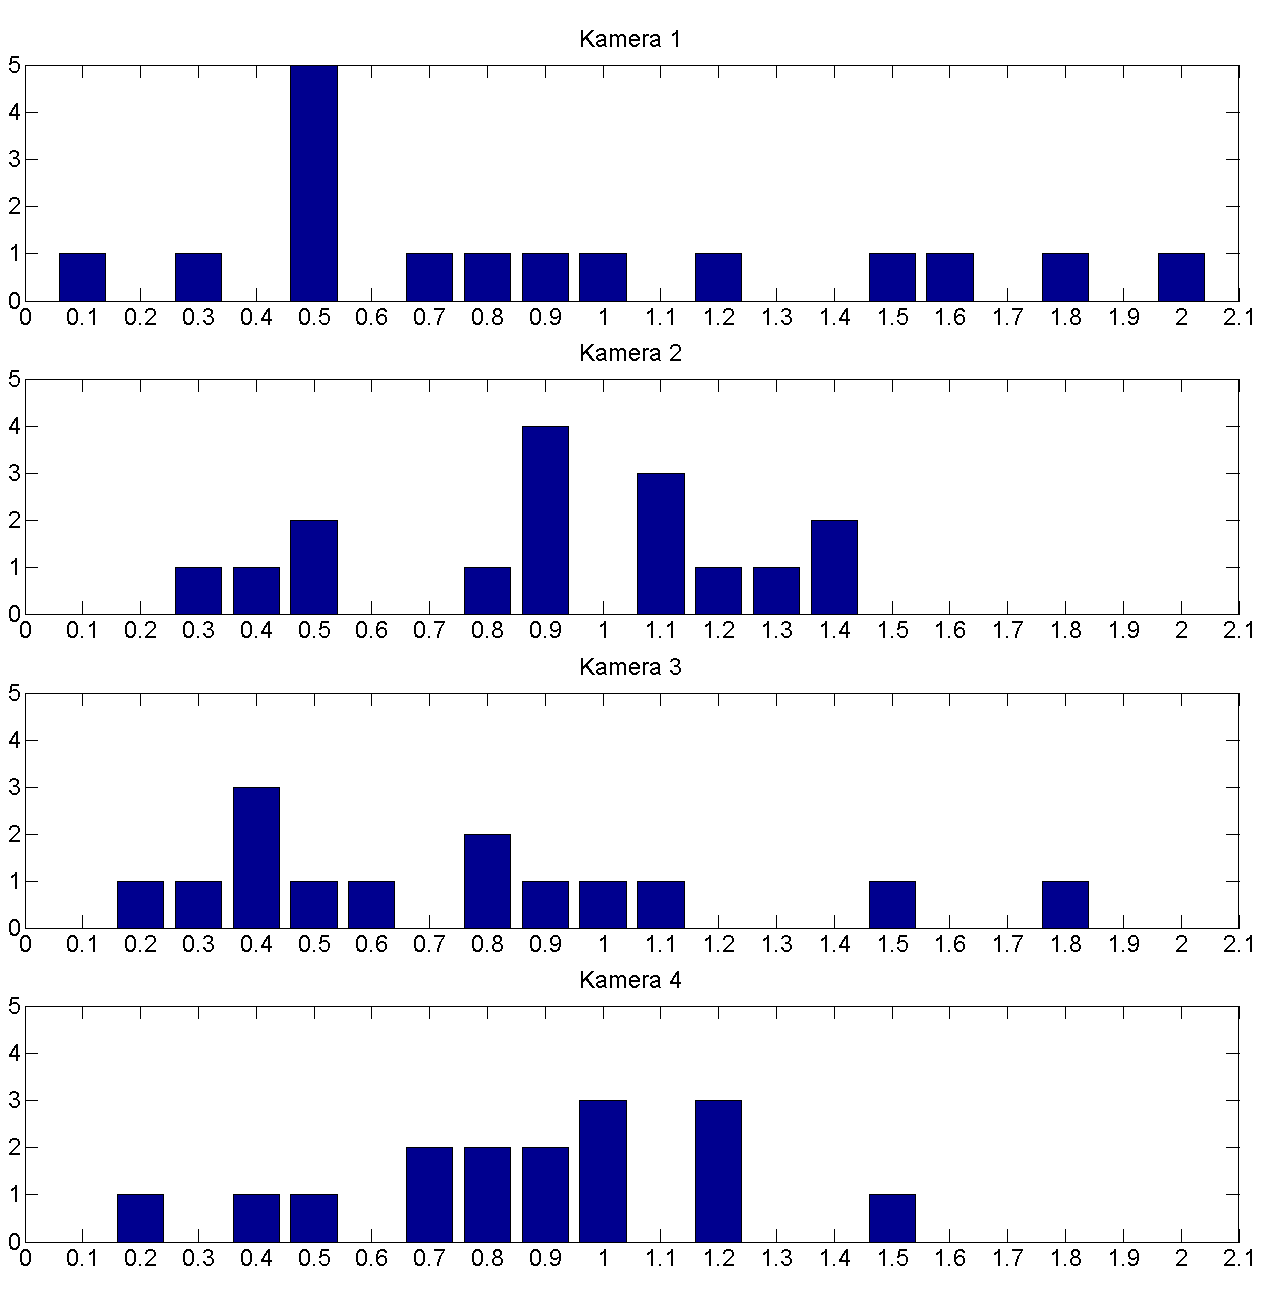
\includegraphics[width=\textwidth,height=\textheight,keepaspectratio]{reprojected_bar.png}
\caption{Histogrami reprojekcijskih napak. Velikost koša je 0.1 slikovnega elementa.}
\end{figure}

\section{Natančnost zaznavanja označevalnika}
Množica podatkov obsega okoli 25 slik označevalnika iz vsake kamere. Skupaj torej okoli 100 slik. Na vseh slikah je bila ročno izbrana sredina označevalnika in ta točka velja za resnico. Ocenjeni sta dve vrsti množic. Prva ima na vseh slikah statično pozicijo označevalnika, saj je bil v času zajemanja slik označevalnik na istem mestu. Zaradi šuma pri zajemu slik pa algoritem za zaznavanje označevalnika ne zazna vedno enako točko na sliki. Povprečje napake je $0,8614$ slikovnega elementa z varianco $0,1899$. Iz spodnjih histogramov se lepo vidi, da je varianca majhna. Slike iz tretje in četrte kamere skoraj vedno določijo enako točko označevalnika. Pri slikah iz prve in druge kamere pa šum povzroči majhno spremembo intenzitet pik, kar posledično zmede algoritem za zaznavanje označevalnika.

\begin{figure}[H]
\centering
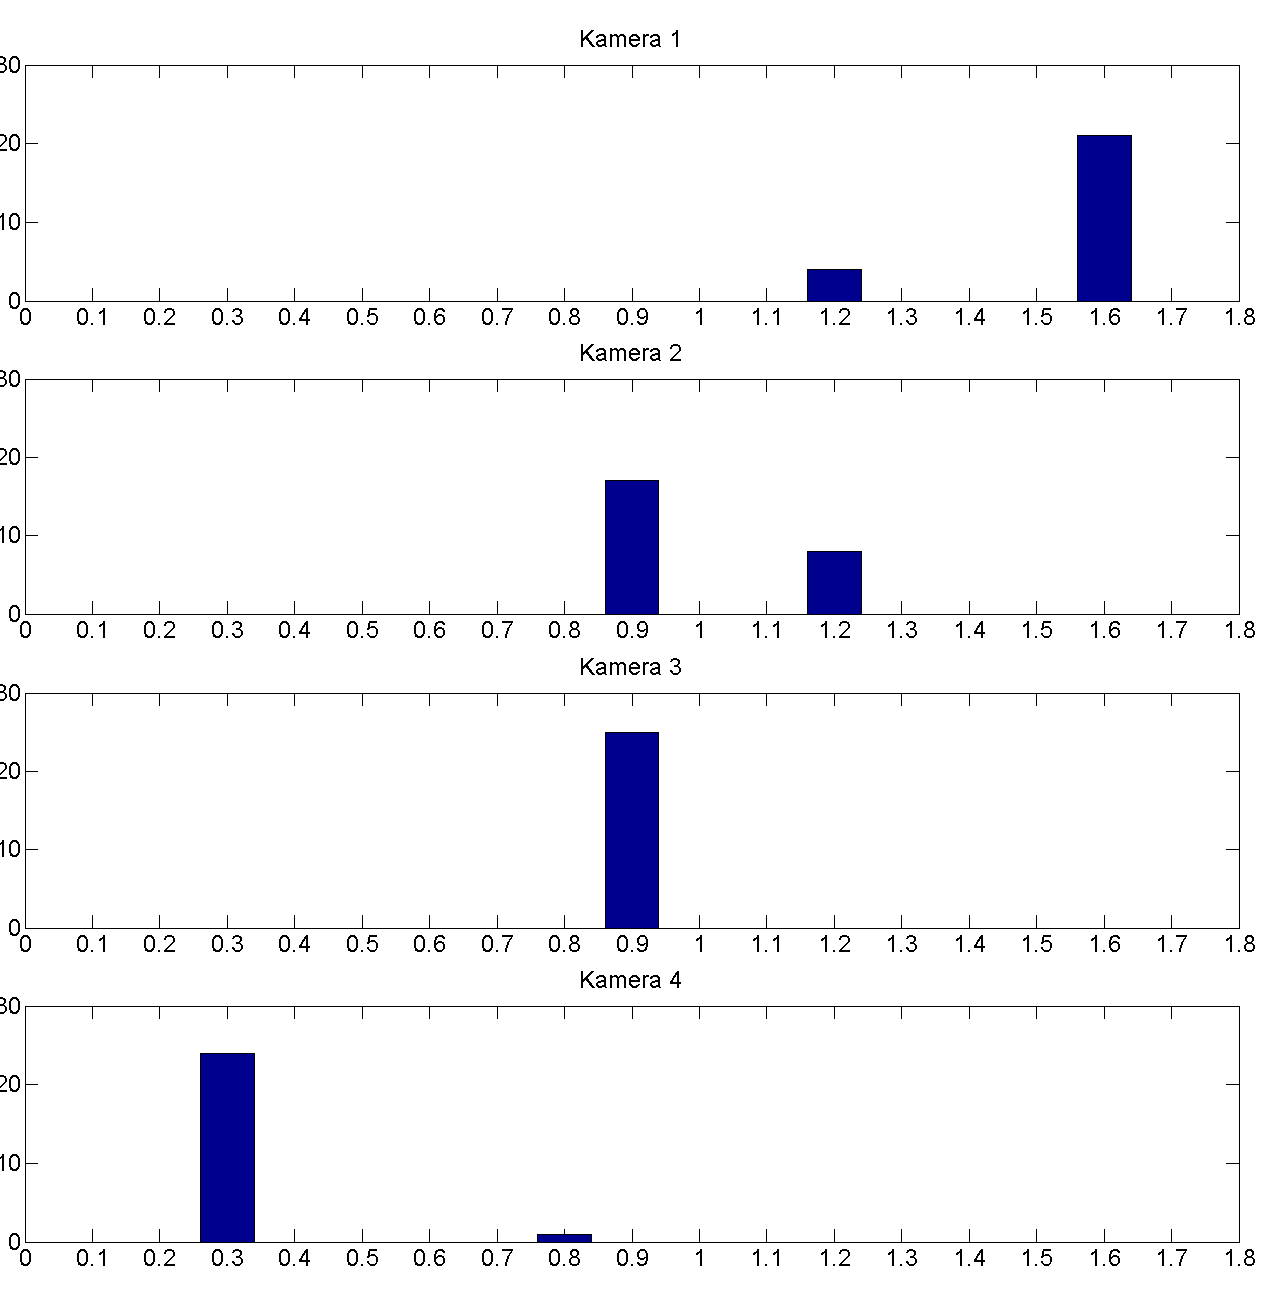
\includegraphics[width=\textwidth,height=\textheight,keepaspectratio]{marker_detection_static_bar.png}
\caption{Histogrami napak zaznavanja statičnega označevalnika.}
\end{figure}

\begin{figure}[H]
\centering
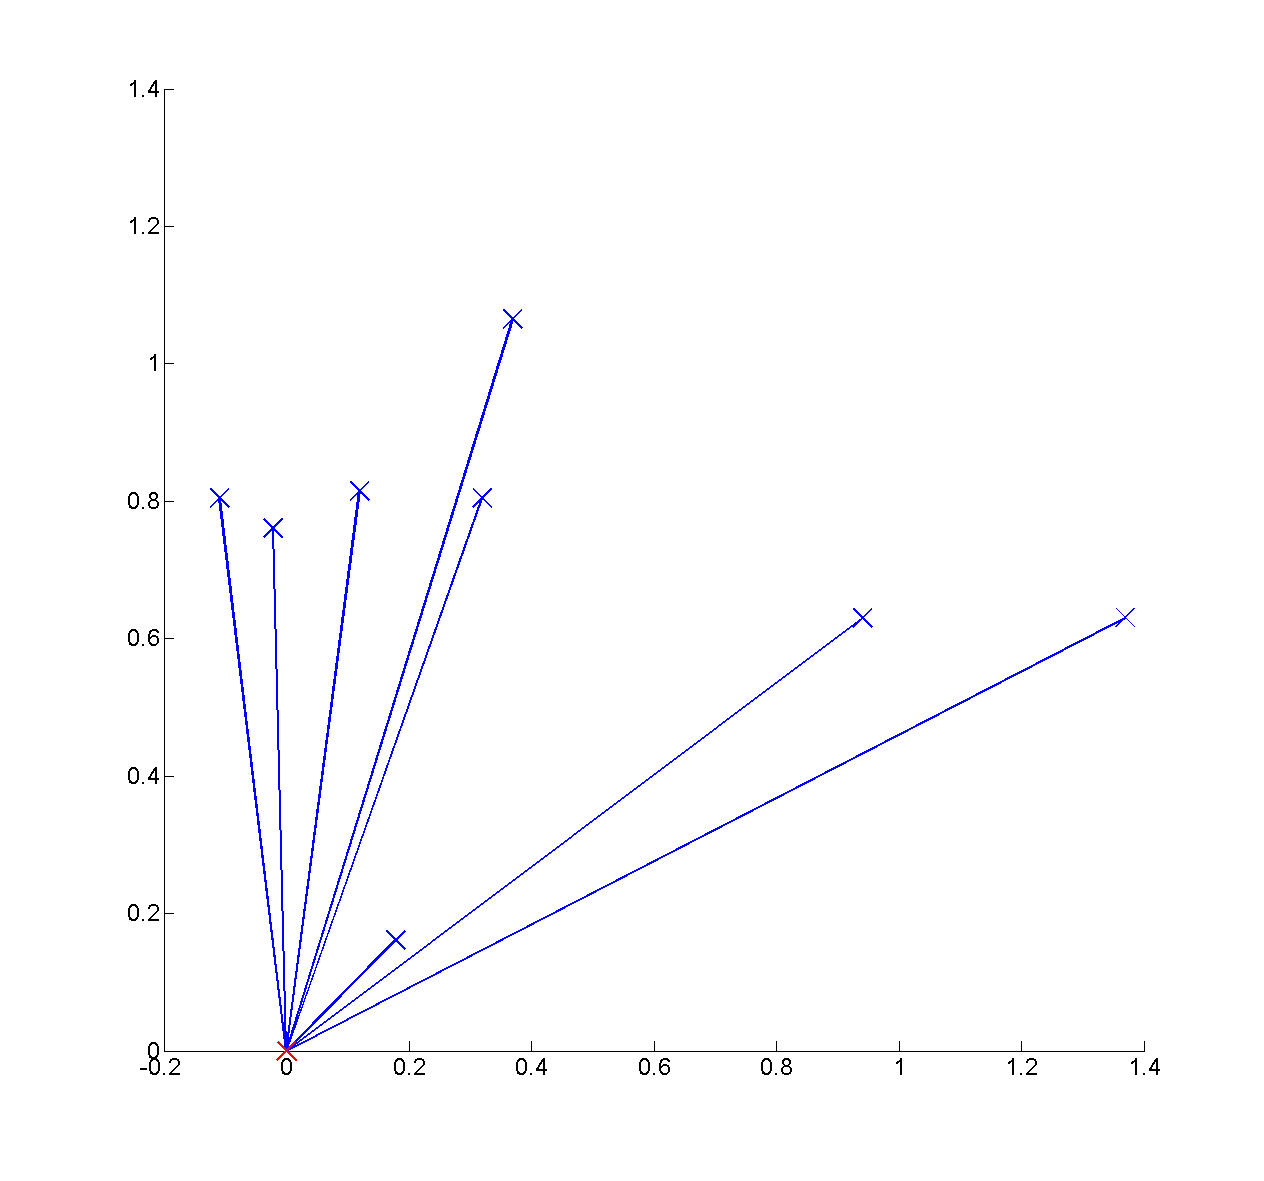
\includegraphics[width=\textwidth,height=\textheight,keepaspectratio]{marker_detection_static_errors.png}
\caption{Graf vektorjev napak. Enote so slikovne pike. Zanimiva je opazka, da so vektorji usmerjeni predvsem v prvi kvadrant.}
\end{figure}

V množici 80 slik pa je označevalnik vsakič na drugem mestu v prosotru (je dinamičen). Povprečje napake je $0,852$ slikovnega elementa z varianco $0,2124$. Iz histogramov vidimo, da je napaka bolj enakomerno porazdeljena kot pri zaznavanju statičnega označevalnika.

\begin{figure}[H]
\centering
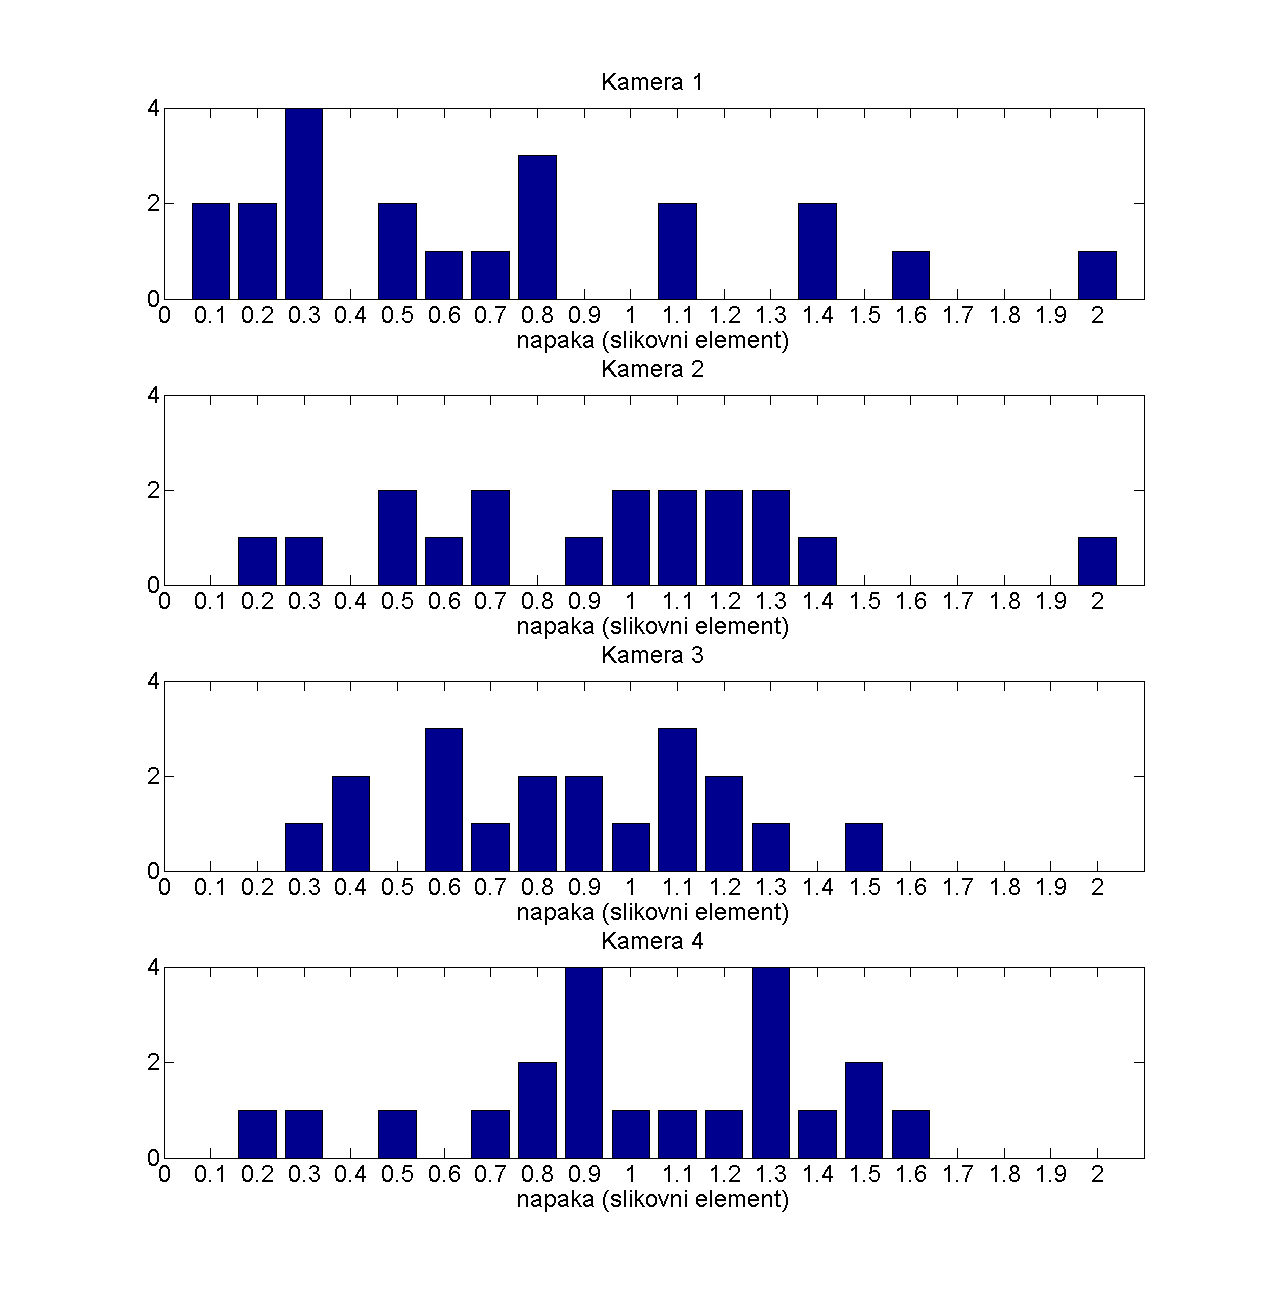
\includegraphics[width=\textwidth,height=\textheight,keepaspectratio]{marker_detection_dynamic_bar.png}
\caption{Histogrami napak zaznavanja dinamičnega označevalnika.}
\end{figure}

\begin{figure}[H]
\centering
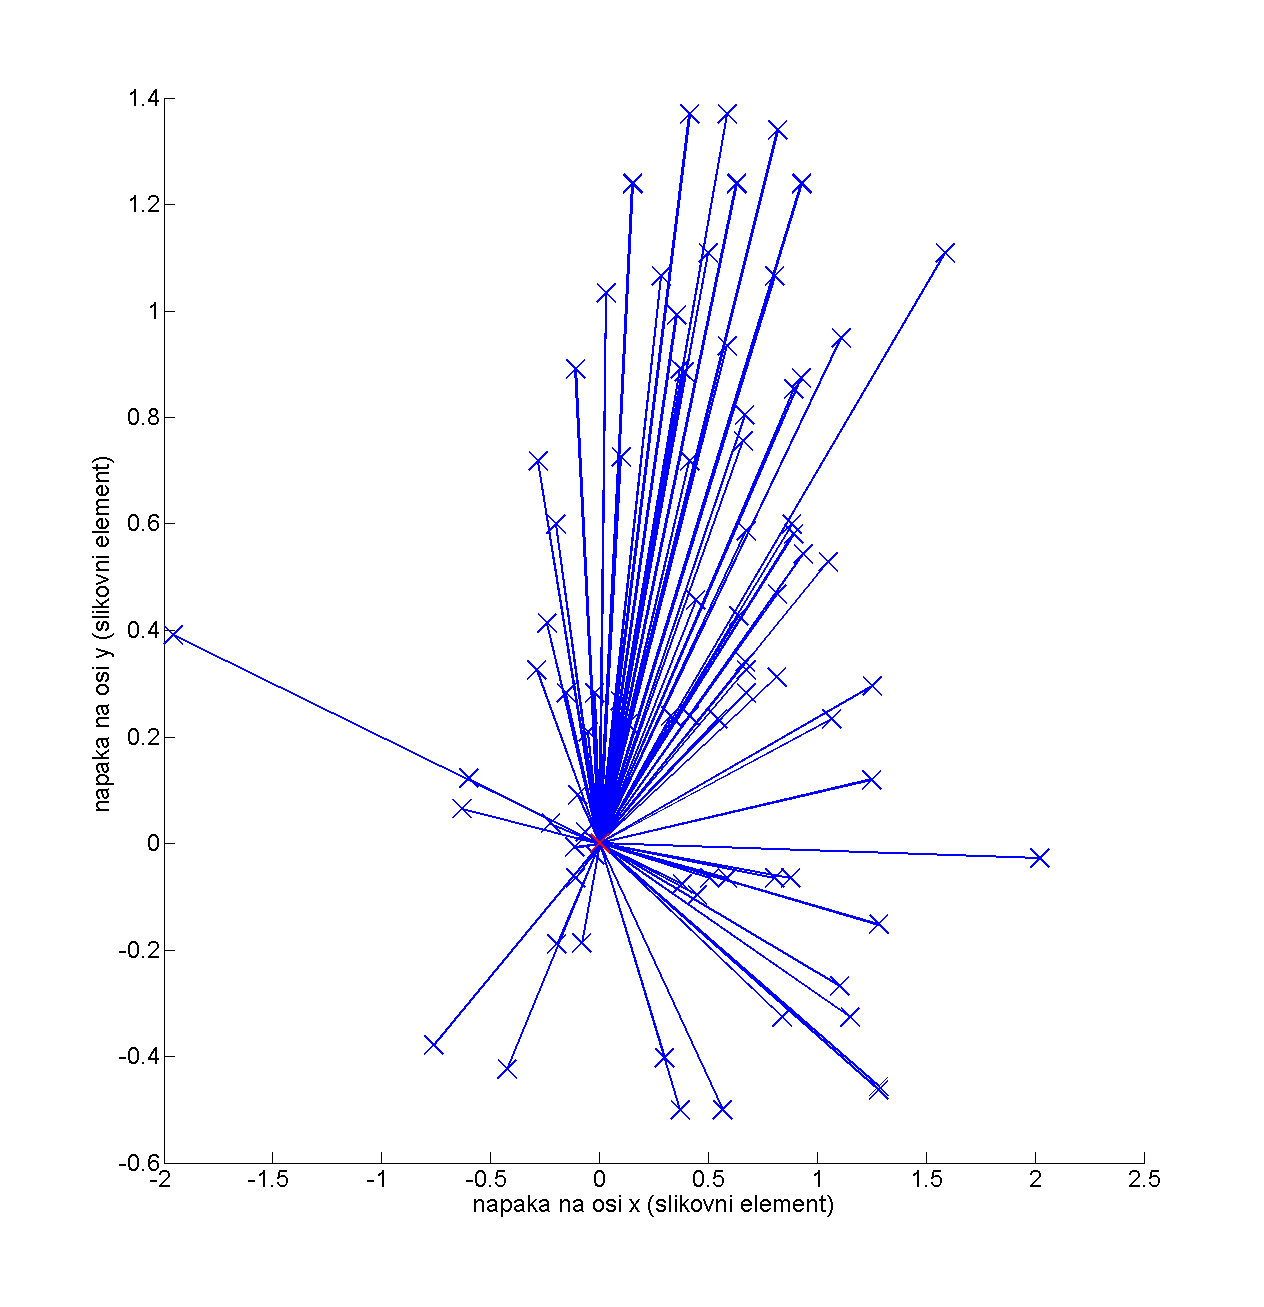
\includegraphics[width=\textwidth,height=\textheight,keepaspectratio]{marker_detection_dynamic_errors.png}
\caption{Graf vektorjev napak. Enota je slikovni element. Gostota zaznanih točk je večja v zgornji polovici grafa, kar je lahko posledica rahle neenakomerne osvetljenosti označevalnika.}
\end{figure}

\section{Natančnost pozicioniranja}
Zunanji parametri kamer so bili kalibrirani s 16 koplanarnimi točkami. Za testiranje natančnosti pa v prostoru izberemo poljubno točko s poznanimi koordinatami. Izbranih je bilo 12 točk v svetu na katerih je bil postavljen označevalnik. Na eni točki je bilo opravljenih več meritev, ki so prikazane v tabeli \ref{positionerrortable}.
\begin{table}[H]
\centering
\begin{tabular}{| c | c | c | c |}
\hline
št. kamer & višina točke (cm) & povprečna napaka (cm) & varianca napake \\
\hline
2 & 2 & 2,3594 & 0,5225 \\
3 & 2 & 1,2737 & 0,1988 \\
4 & 2 & 1,2146 & 0,6575 \\

2 & 62,6 & 3,4443 & 5,1579 \\
3 & 62,6 & 3,8677 & 2,3627 \\
4 & 62,6 & 8,7621 & 21,4037 \\
\hline
\end{tabular}
\caption{}
\label{positionerrortable}
\end{table}


\chapter{Zaključek}

\bibliography{bibliography}{}
\bibliographystyle{plain}
\end{document}

